\documentclass[a4paper,14pt]{extarticle}
\usepackage[left=2.5cm, right=1.5cm, vmargin=2.5cm]{geometry}
\usepackage[utf8]{inputenc}
\usepackage[T2A]{fontenc}
\usepackage[russian]{babel}
\usepackage{graphicx}
\graphicspath{{pictures/}}
\usepackage{caption}
\usepackage{subcaption}
\usepackage{indentfirst}
\setlength\parindent{5ex}
\usepackage{fancyhdr}
\usepackage{booktabs}
\usepackage{siunitx} 
\usepackage{pgfplotstable}
\usepackage{amsmath}
\usepackage{autonum}
\usepackage{amsfonts}
\DeclareMathOperator{\sign}{sgn}
\newcommand{\gt}{\textgreater} % знак больше
\newcommand{\lt}{\textless}       % знак меньше
\DeclareGraphicsExtensions{.pdf,.png,.jpg}
\pagestyle{fancy}
\fancyhf{}
\rhead{\thepage}
\renewcommand{\headrulewidth}{0pt}

\fancypagestyle{plain}{ 
	\fancyhf{}
	\rhead{\thepage}}

\author{Никитин Илья}

\title{Отчет по лабораторной работе №3: "Тепловые свойства твердых тел"}
\date{\today}

\begin{document}
	
	\maketitle
	\tableofcontents

	\section{Задачи}
		Определить температурную зависимость сопротивления, а также коэффициенты теплового излучения и теплопередачи в воздух от проволок из разных материалов
	\section{Оборудование}
		\begin{itemize}
			\item Проволоки из различных материалов
			\item Термопаста КПТ-19
			\item Алюминевая банка
			\item Термопара К-типа
			\item Мультиметр
			\item Шунт
			\item Два мультиметра Keysight
			\item Коробка картонная
			\item Клемник
			\item Компьютер с программой LabView
			\item Электрический кипятильник
			\item Источник тока Gophert
			\item Резинки для зажима проволоки
		\end{itemize}
	\section{Теория}
		\subsection{Температурная зависимость удельного сопротивления металлов}
			В этой работе будут использоваться материалы, состоящие из простых веществ: медь, титан, вольфрам. Все эти материалы при нормальных условиях являются классическими примерами твердых тел -- металлов. Их общее свойство состоит в линейной зависимости удельного сопротивления от температуры:
			\begin{equation}
				\rho = \rho_0 [1 + \alpha(T - T_0)]
				\end{equation}
		\subsection{Теплоотдача}
			Процесс теплоотдачи описывается эмпирическим законом Ньютона-Рихмана, согласно которому нормальная компонента потока тепла через стенку твердого тела наружу пропорциональа разности температур тела и среды:
			\begin{equation}
				q_n = \beta (T - T_0)
			\end{equation}
		\subsection{Тепловое излучение}
			Согласно закону Стефана-Больцмана мощность теплового узлучения с небольшой площадки DS на поверхности тела, имеющего абсолютную температуру T, пропорциональна разности четвертой степени температур тела и окружающей среды:
			\begin{equation}
				dP = \epsilon \sigma (T^4 - T^4_0)dS
			\end{equation}
			где $\sigma = \frac{2 \pi^5 k^4_B}{15h^3c^2}$
		\subsection{Мощность}
			В стационарном режиме вся установившаяся мощность $P_{st} = I^2 R_{st}$ равна суммарной мощности тепловых потерь:
			\begin{equation}
				P_{st} = \beta S_{surf} (T - T_0) + \epsilon \sigma S_{surf} (T^4 - T^4_0)
			\end{equation}
	\section{Температурная зависимость сопротивления}
		\subsection{Ход работы}
		Для измерения температурной зависимости сопротивления различных проволок была взята алюминевая банка с водой, кипятильник, термопаста и соответсвующие кусочки проволоки. Проволока обматывалась на банку, предварительно смазанную термопастой, затем проволока подключалась к электрической цепи, в которой измерялся ток и напряжение на проволоке. Кипятильником вода нагревалась шагами по $5 - 10 \circ C$ и  при установлении постоянного тока записывались показания вольтметров, чтобы потом из этих данных получить сопротивление.
			\begin{figure}[h!]
				\centering
				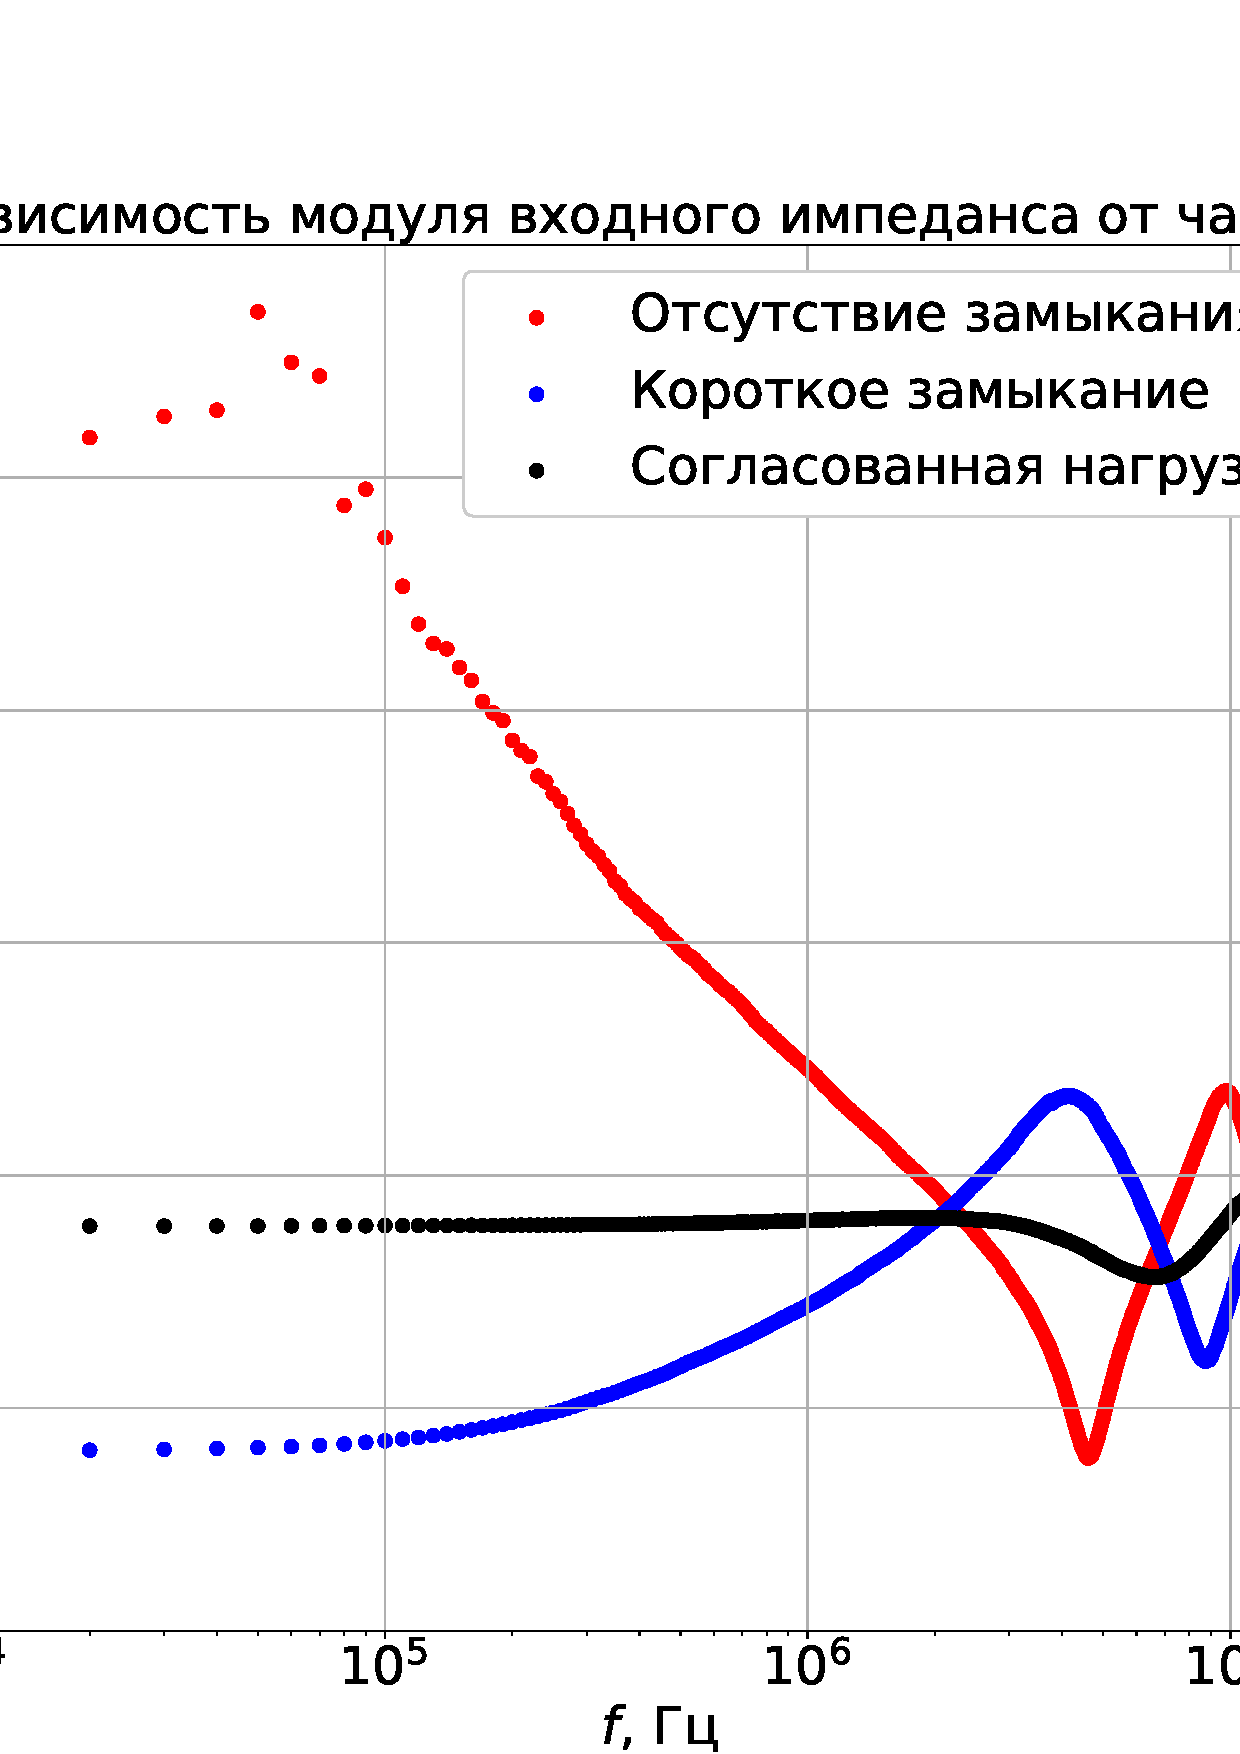
\includegraphics[width=.55\linewidth]{Lab3_1.png}
				\caption{Схема подключения проволоки}
				\label{fig1}
			\end{figure}
		\newpage
		\subsection{Обработка данных}
			\begin{figure}[h!]
				\centering
				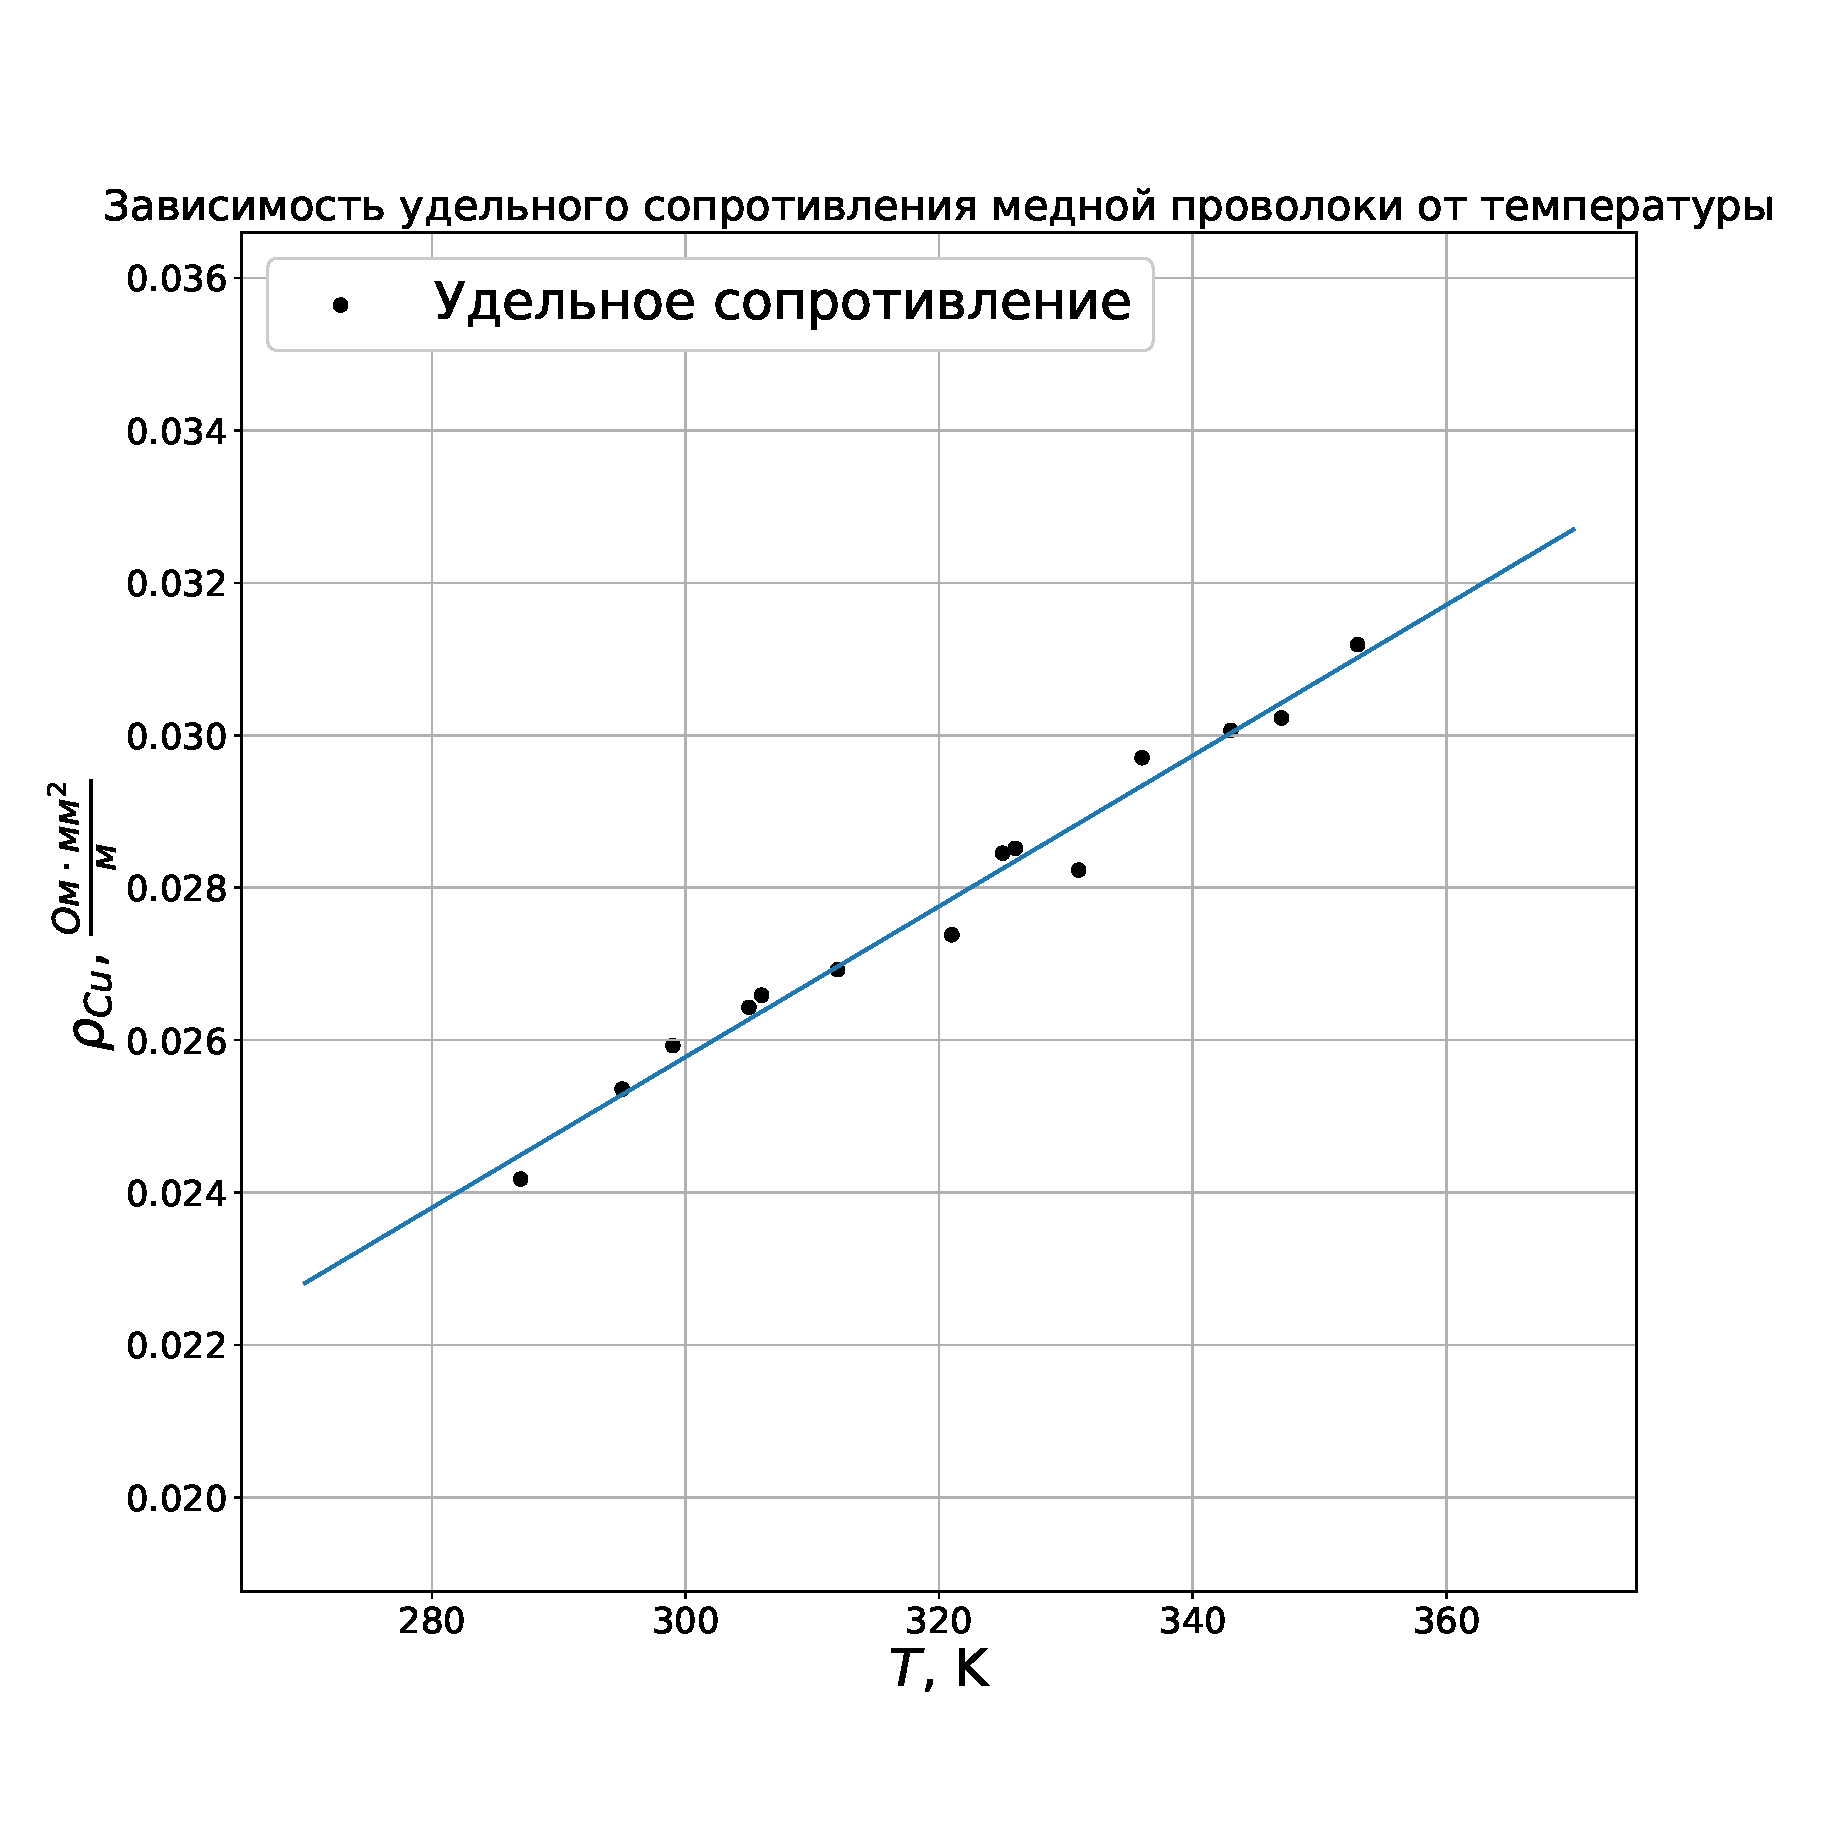
\includegraphics[width=.60\linewidth]{Lab3_2.eps}
				\caption{Получившийся коэффициент температурной зависимости сопротивления $\alpha \approx 3.9 \cdot 10^{-3}$ $\frac{1}{K}$ }
				\label{fig2}
			\end{figure}
		\newpage
			\begin{figure}[h!]
				\centering
				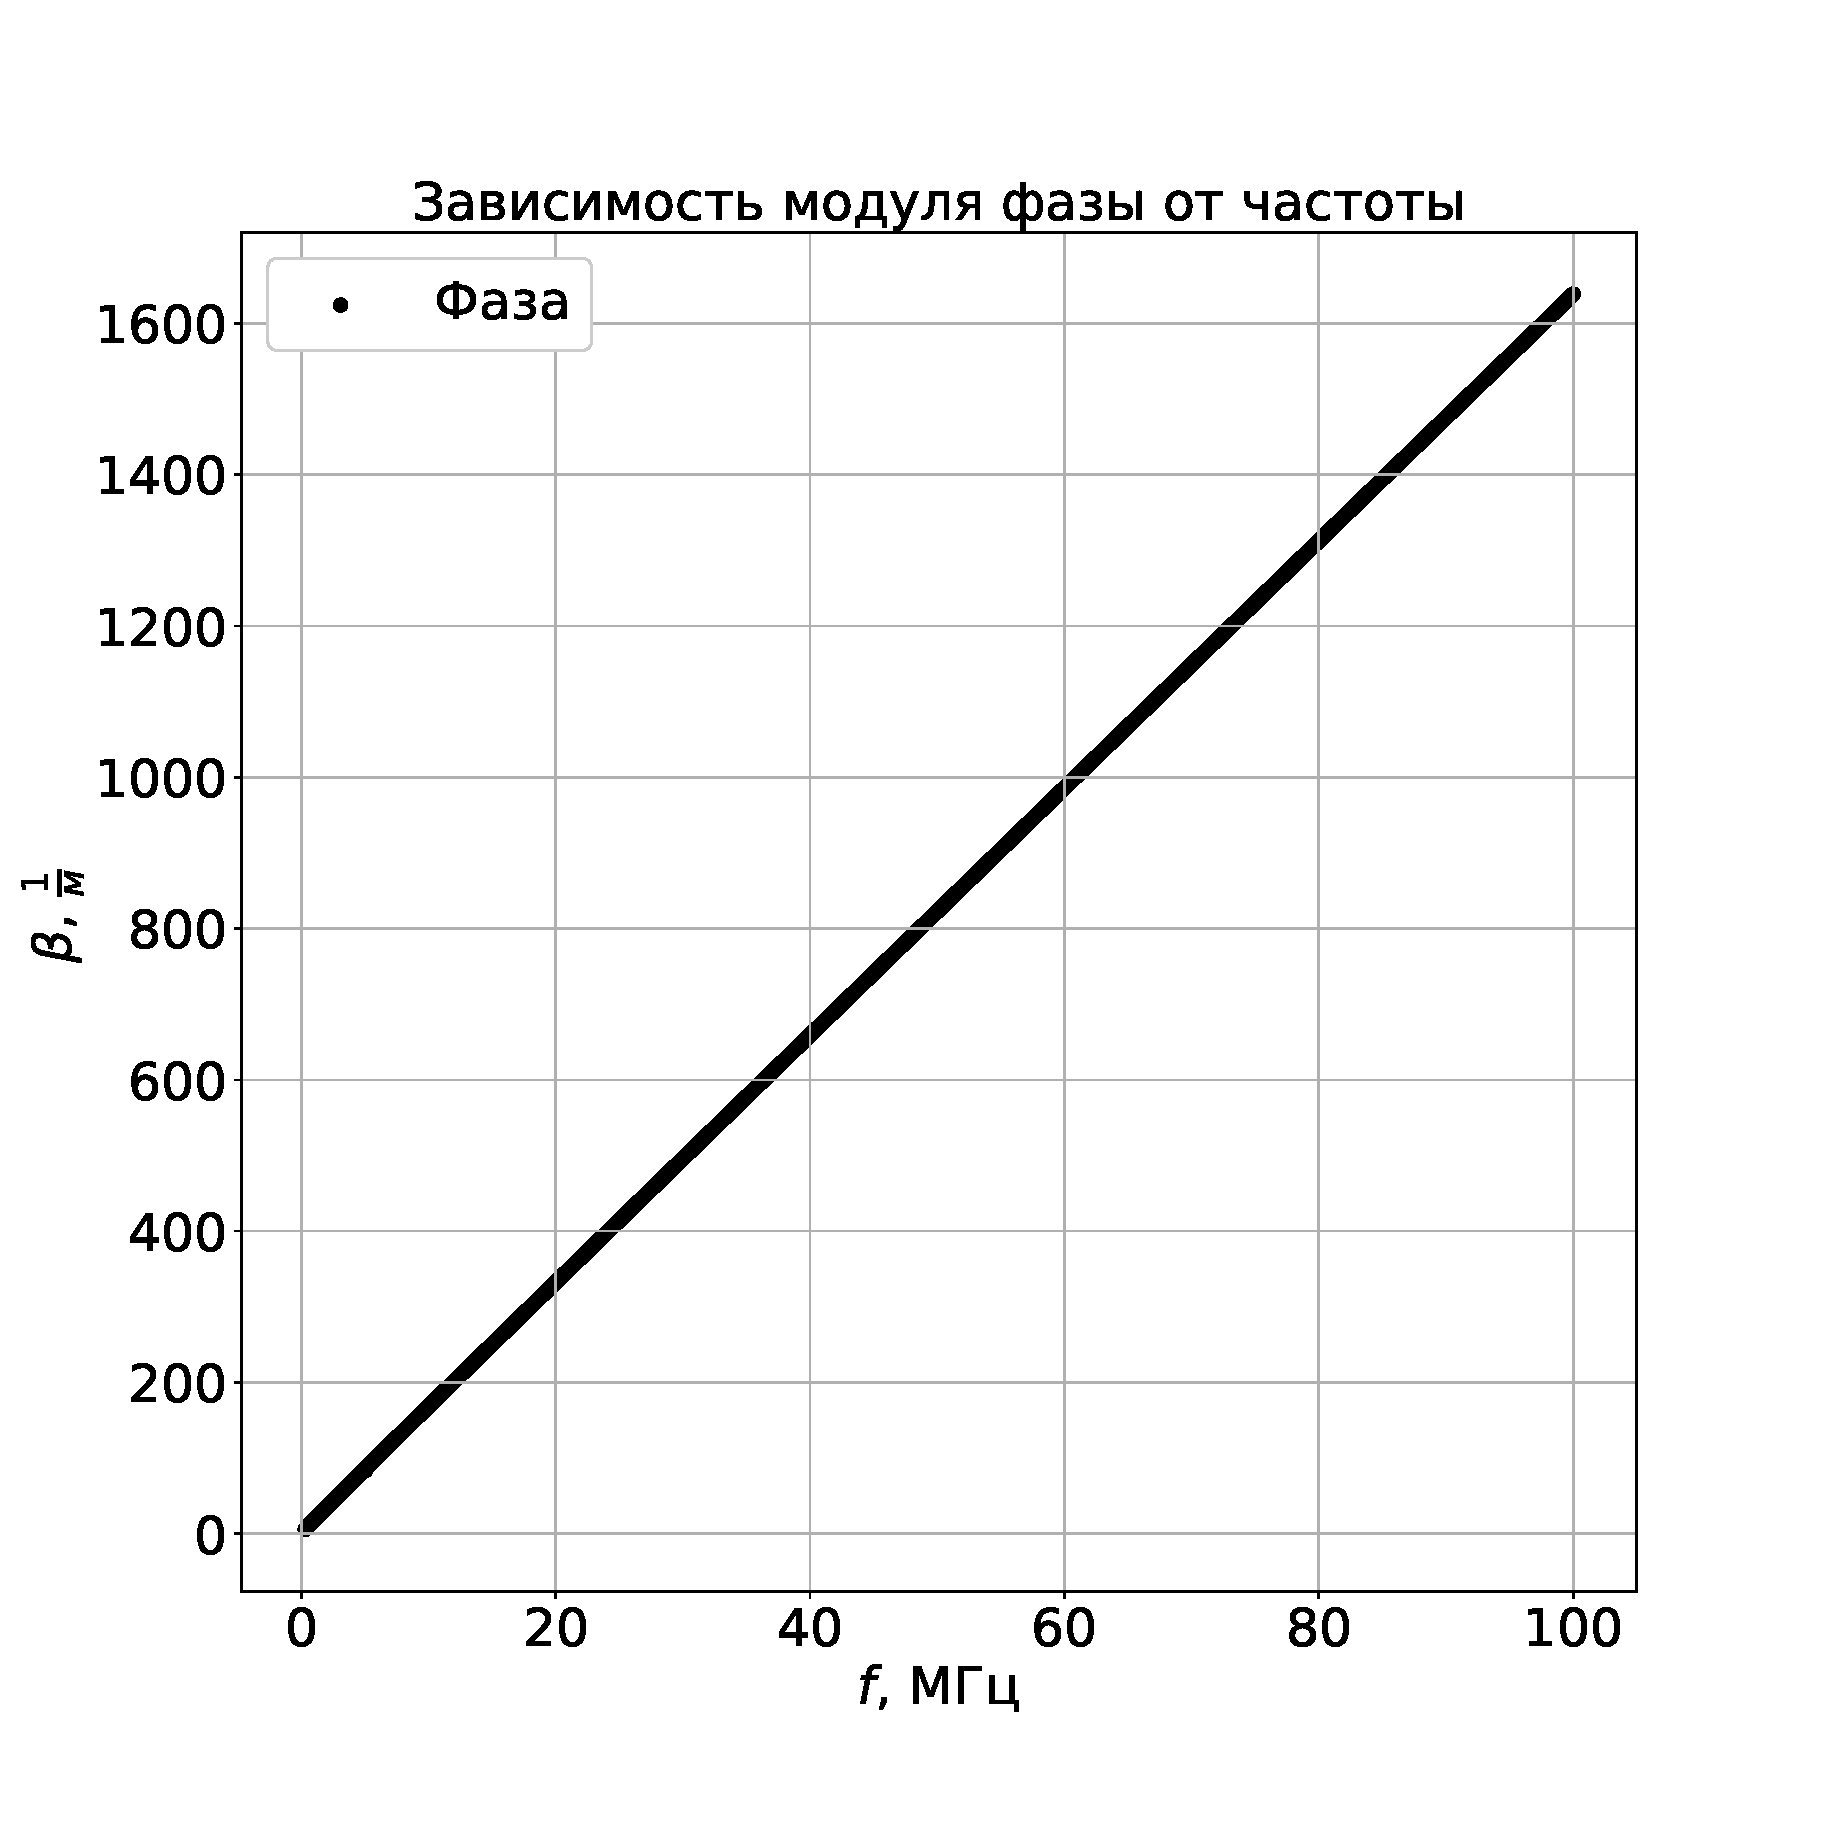
\includegraphics[width=.55\linewidth]{Lab3_3.eps}
				\caption{Получившийся коэффициент температурной зависимости сопротивления $\alpha \approx 127.6 \cdot 10^{-3}$ $\frac{1}{K}$}
				\label{fig3}
			\end{figure}
			\begin{figure}[h!]
				\centering
				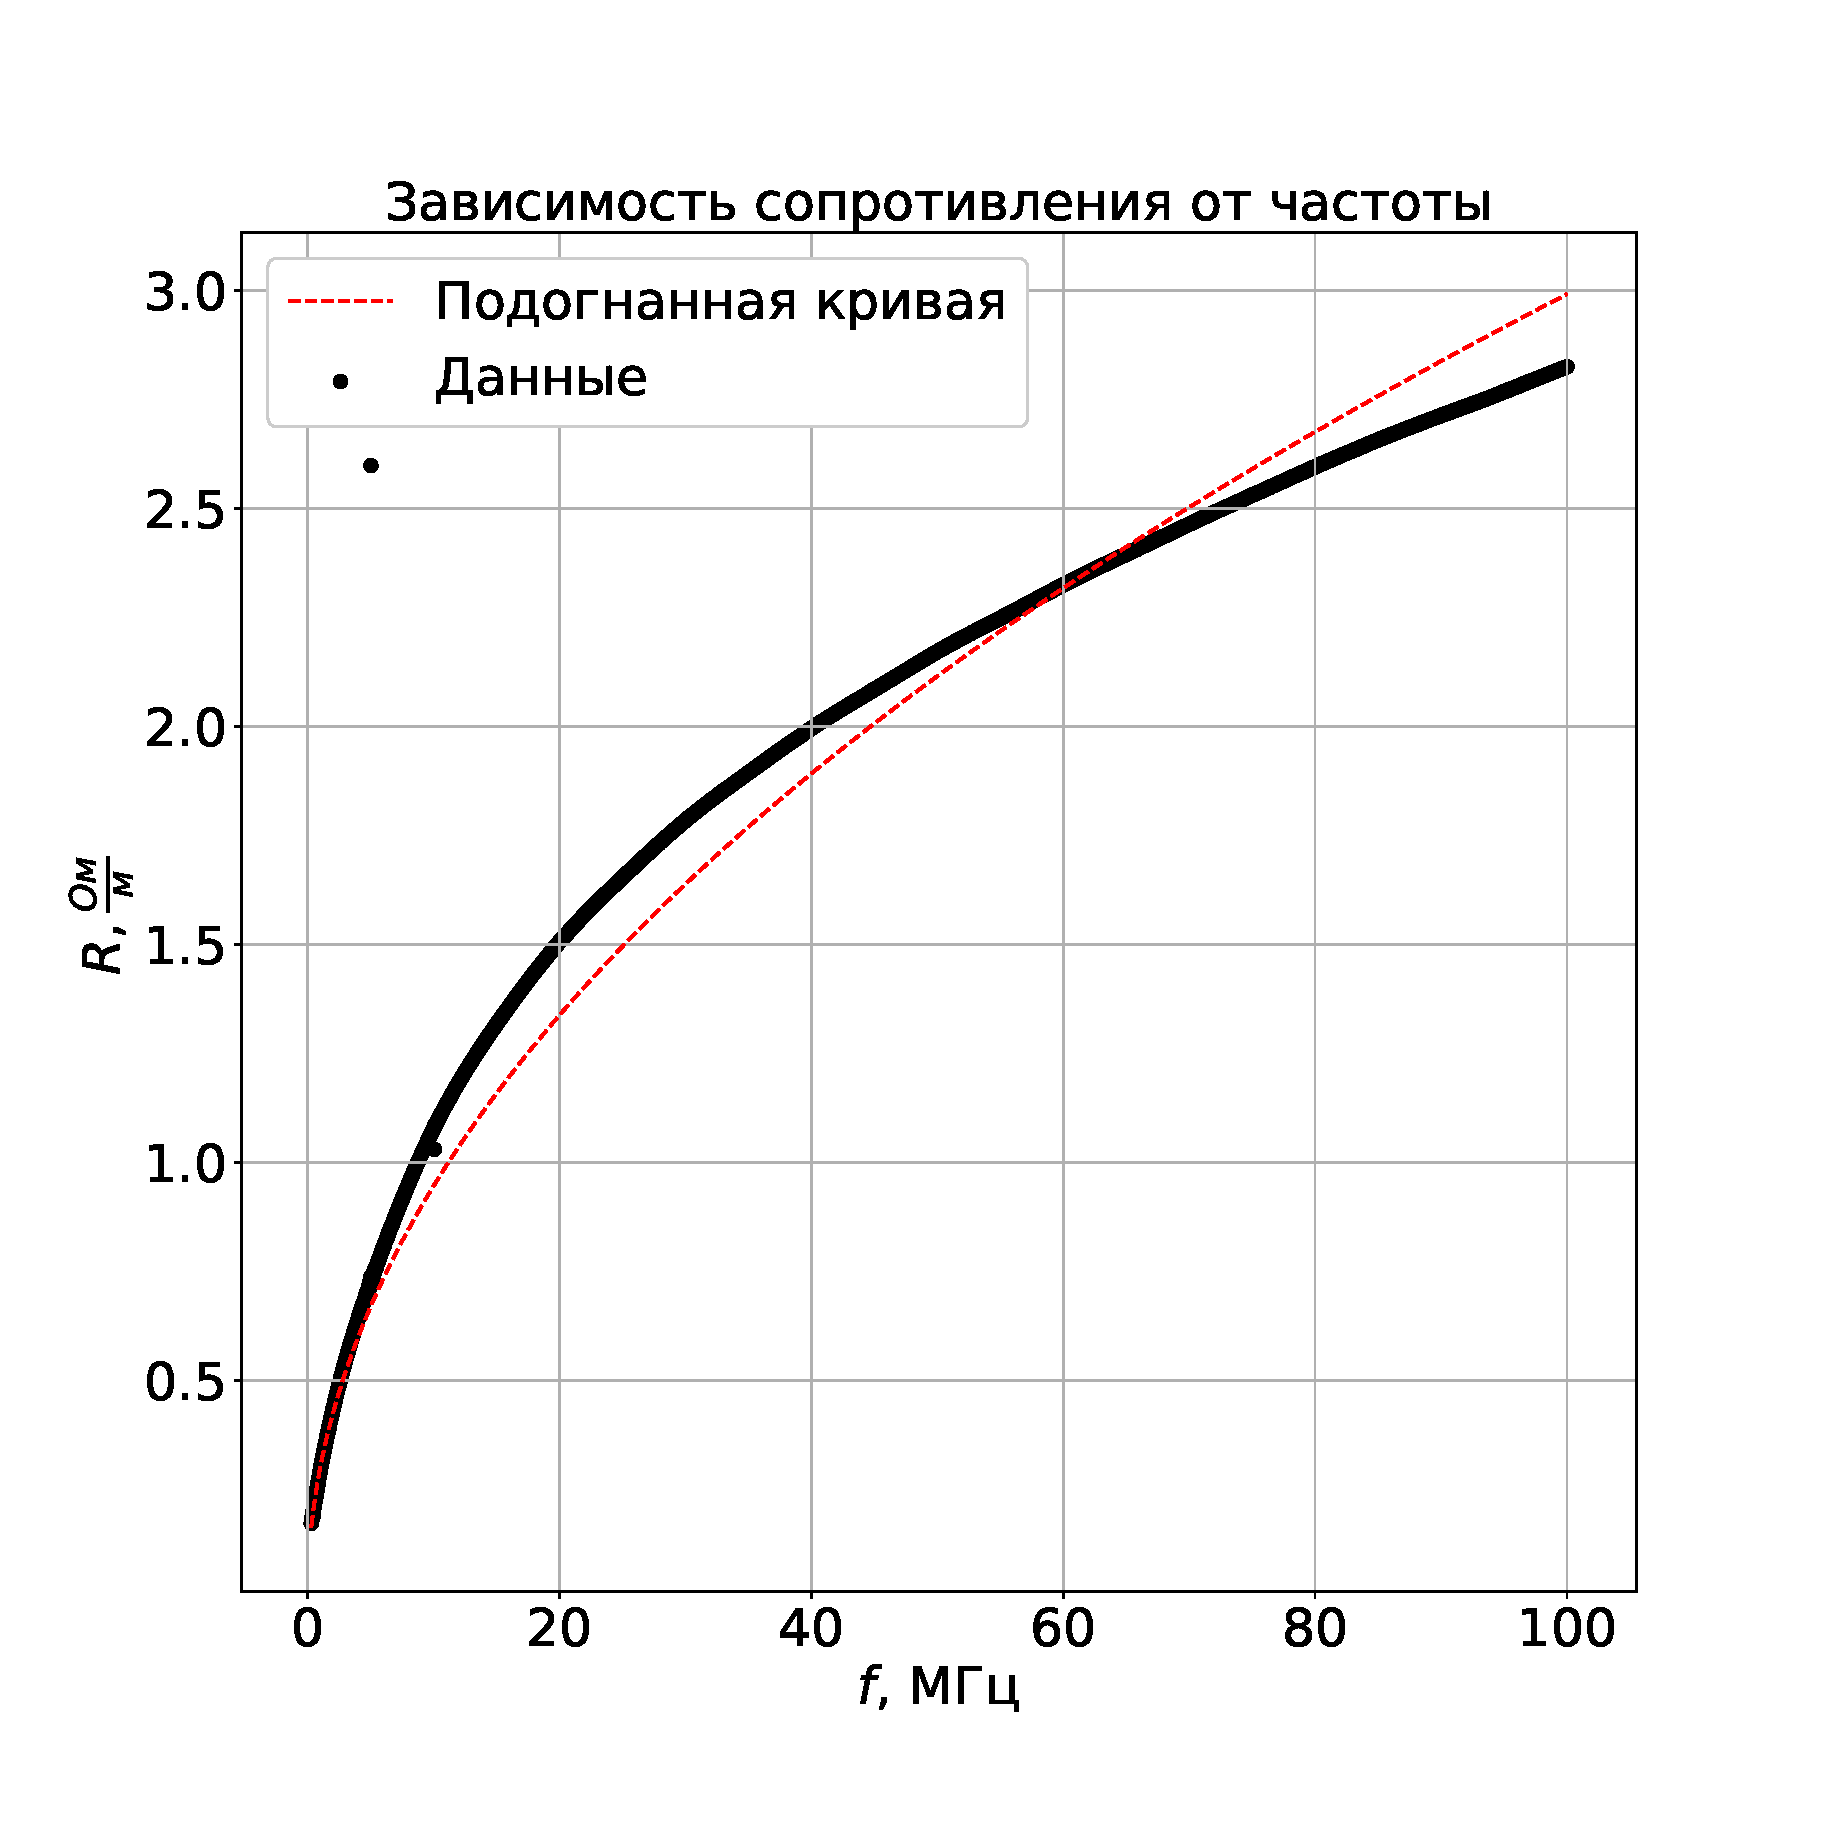
\includegraphics[width=.60\linewidth]{Lab3_4.eps}
				\caption{Получившийся коэффициент температурной зависимости сопротивления $\alpha \approx 2.3 \cdot 10^{-3}$ $\frac{1}{K}$}
				\label{fig4}
			\end{figure}
	\section{Определение мощности потерь и теплоемкости}
		\subsection{Ход работы}
			Для измерения мощности потерь использовалась похожая схема, но без банки, термопары и кипятильника. Проволока в данном случае висела в воздухе и грелась до больших температур за счет подаваемой мощности. Над схемой была установлена картонная коробка, чтобы минимизировать конвективные потоки воздуха.
			\begin{figure}[h!]
				\centering
				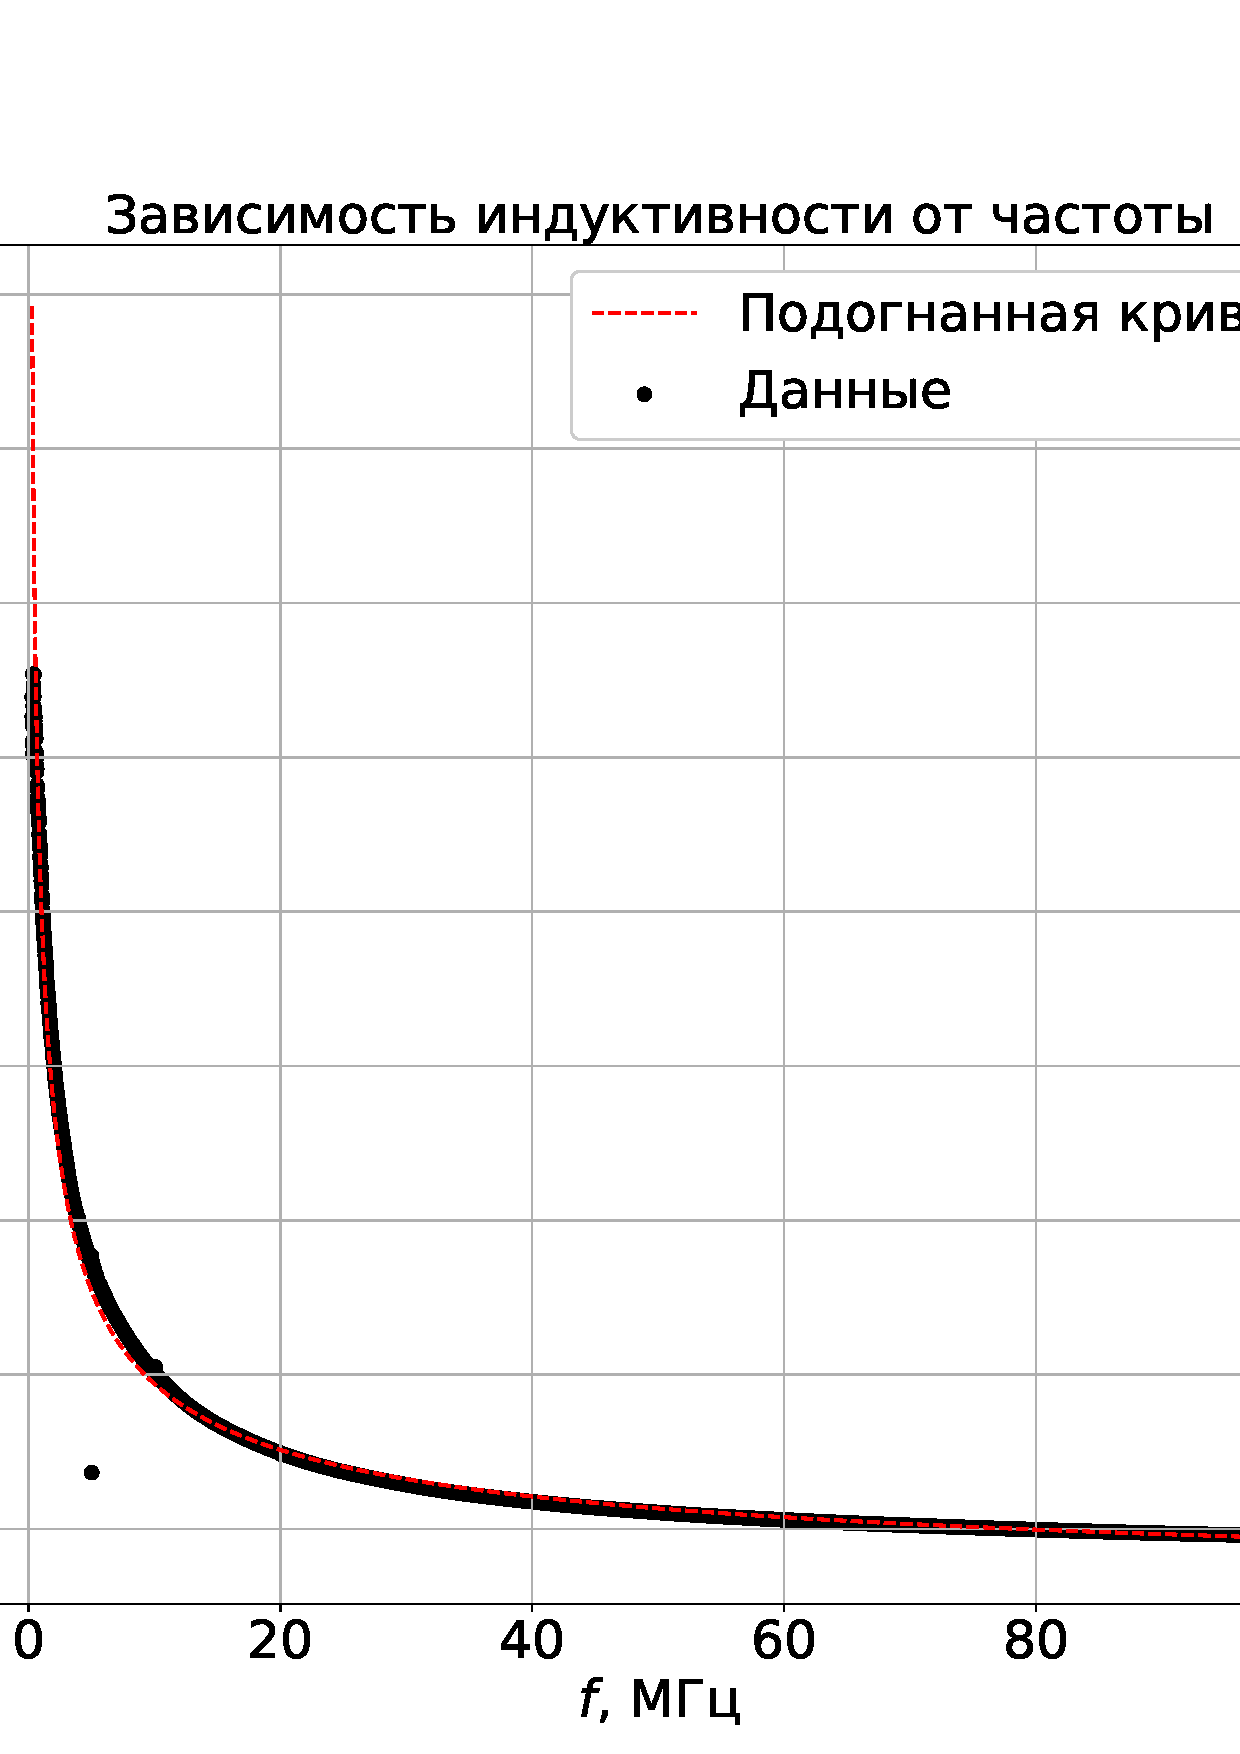
\includegraphics[width=.40\linewidth]{Lab3_5.png}
				\caption{Cхема подключения проволоки}
				\label{fig5}
			\end{figure}
		\subsection{Обработка данных}
			\begin{figure}[h!]
				\centering
				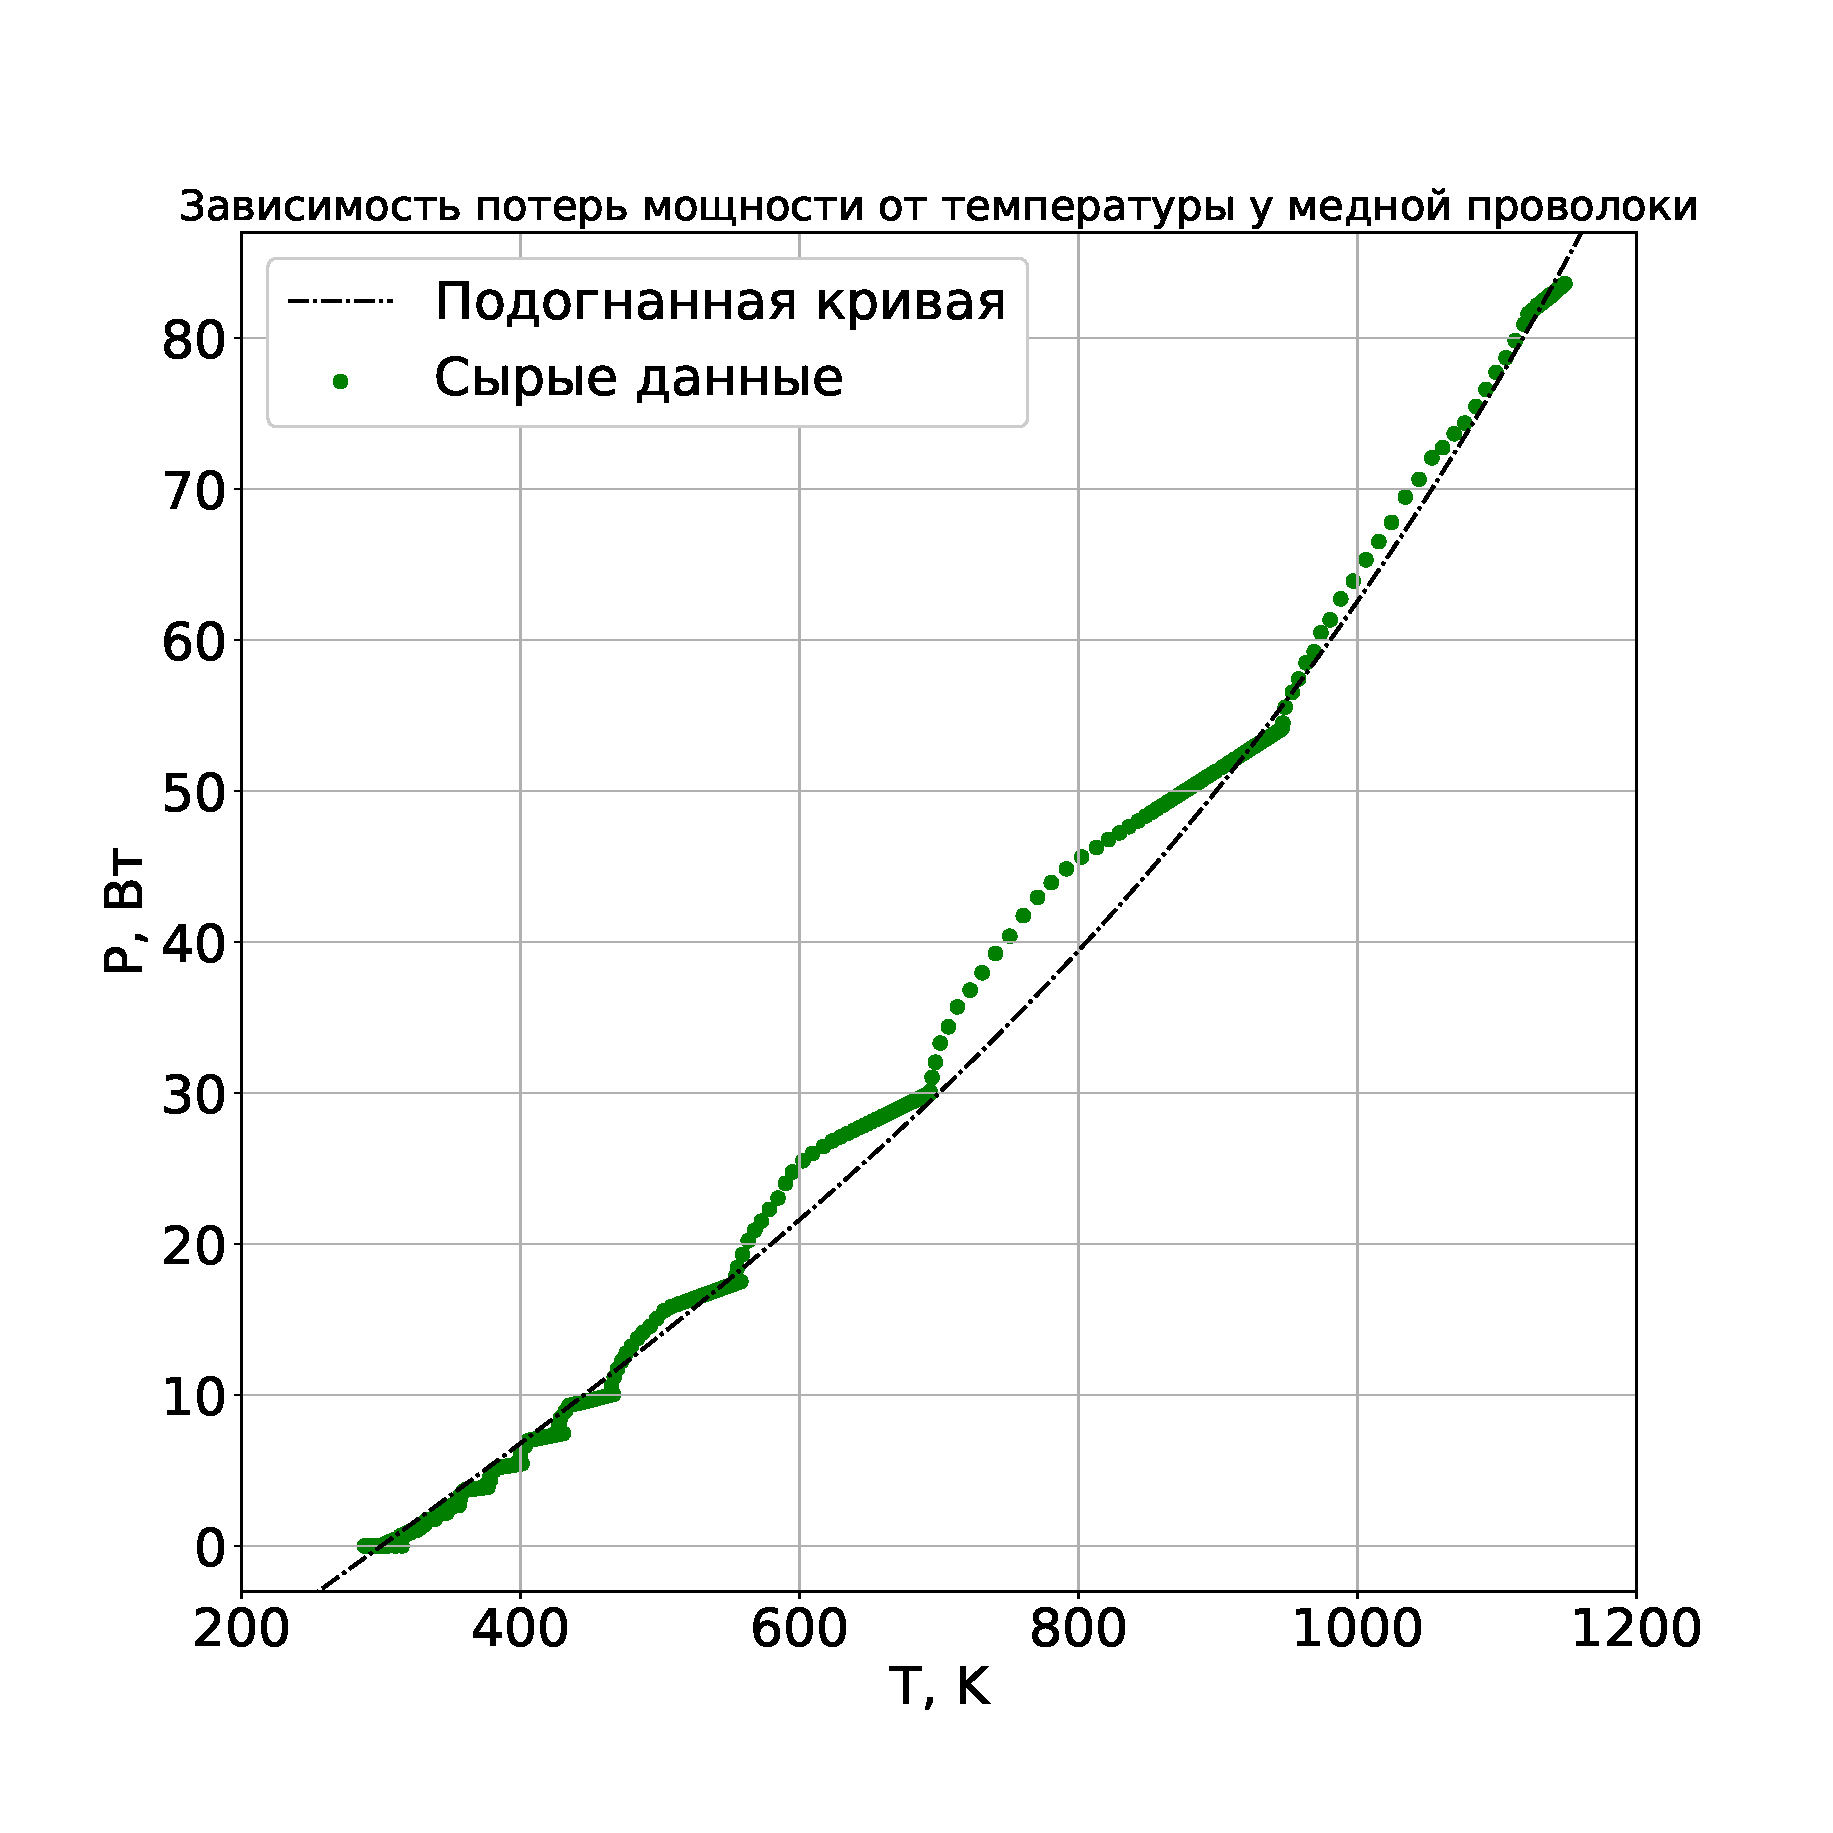
\includegraphics[width=.55\linewidth]{Lab3_6.eps}
				\caption{Коэффициенты $\beta \approx 52.9$, $\epsilon \approx 0.24$}
				\label{fig6}
			\end{figure}
			\begin{figure}[h!]
				\centering
				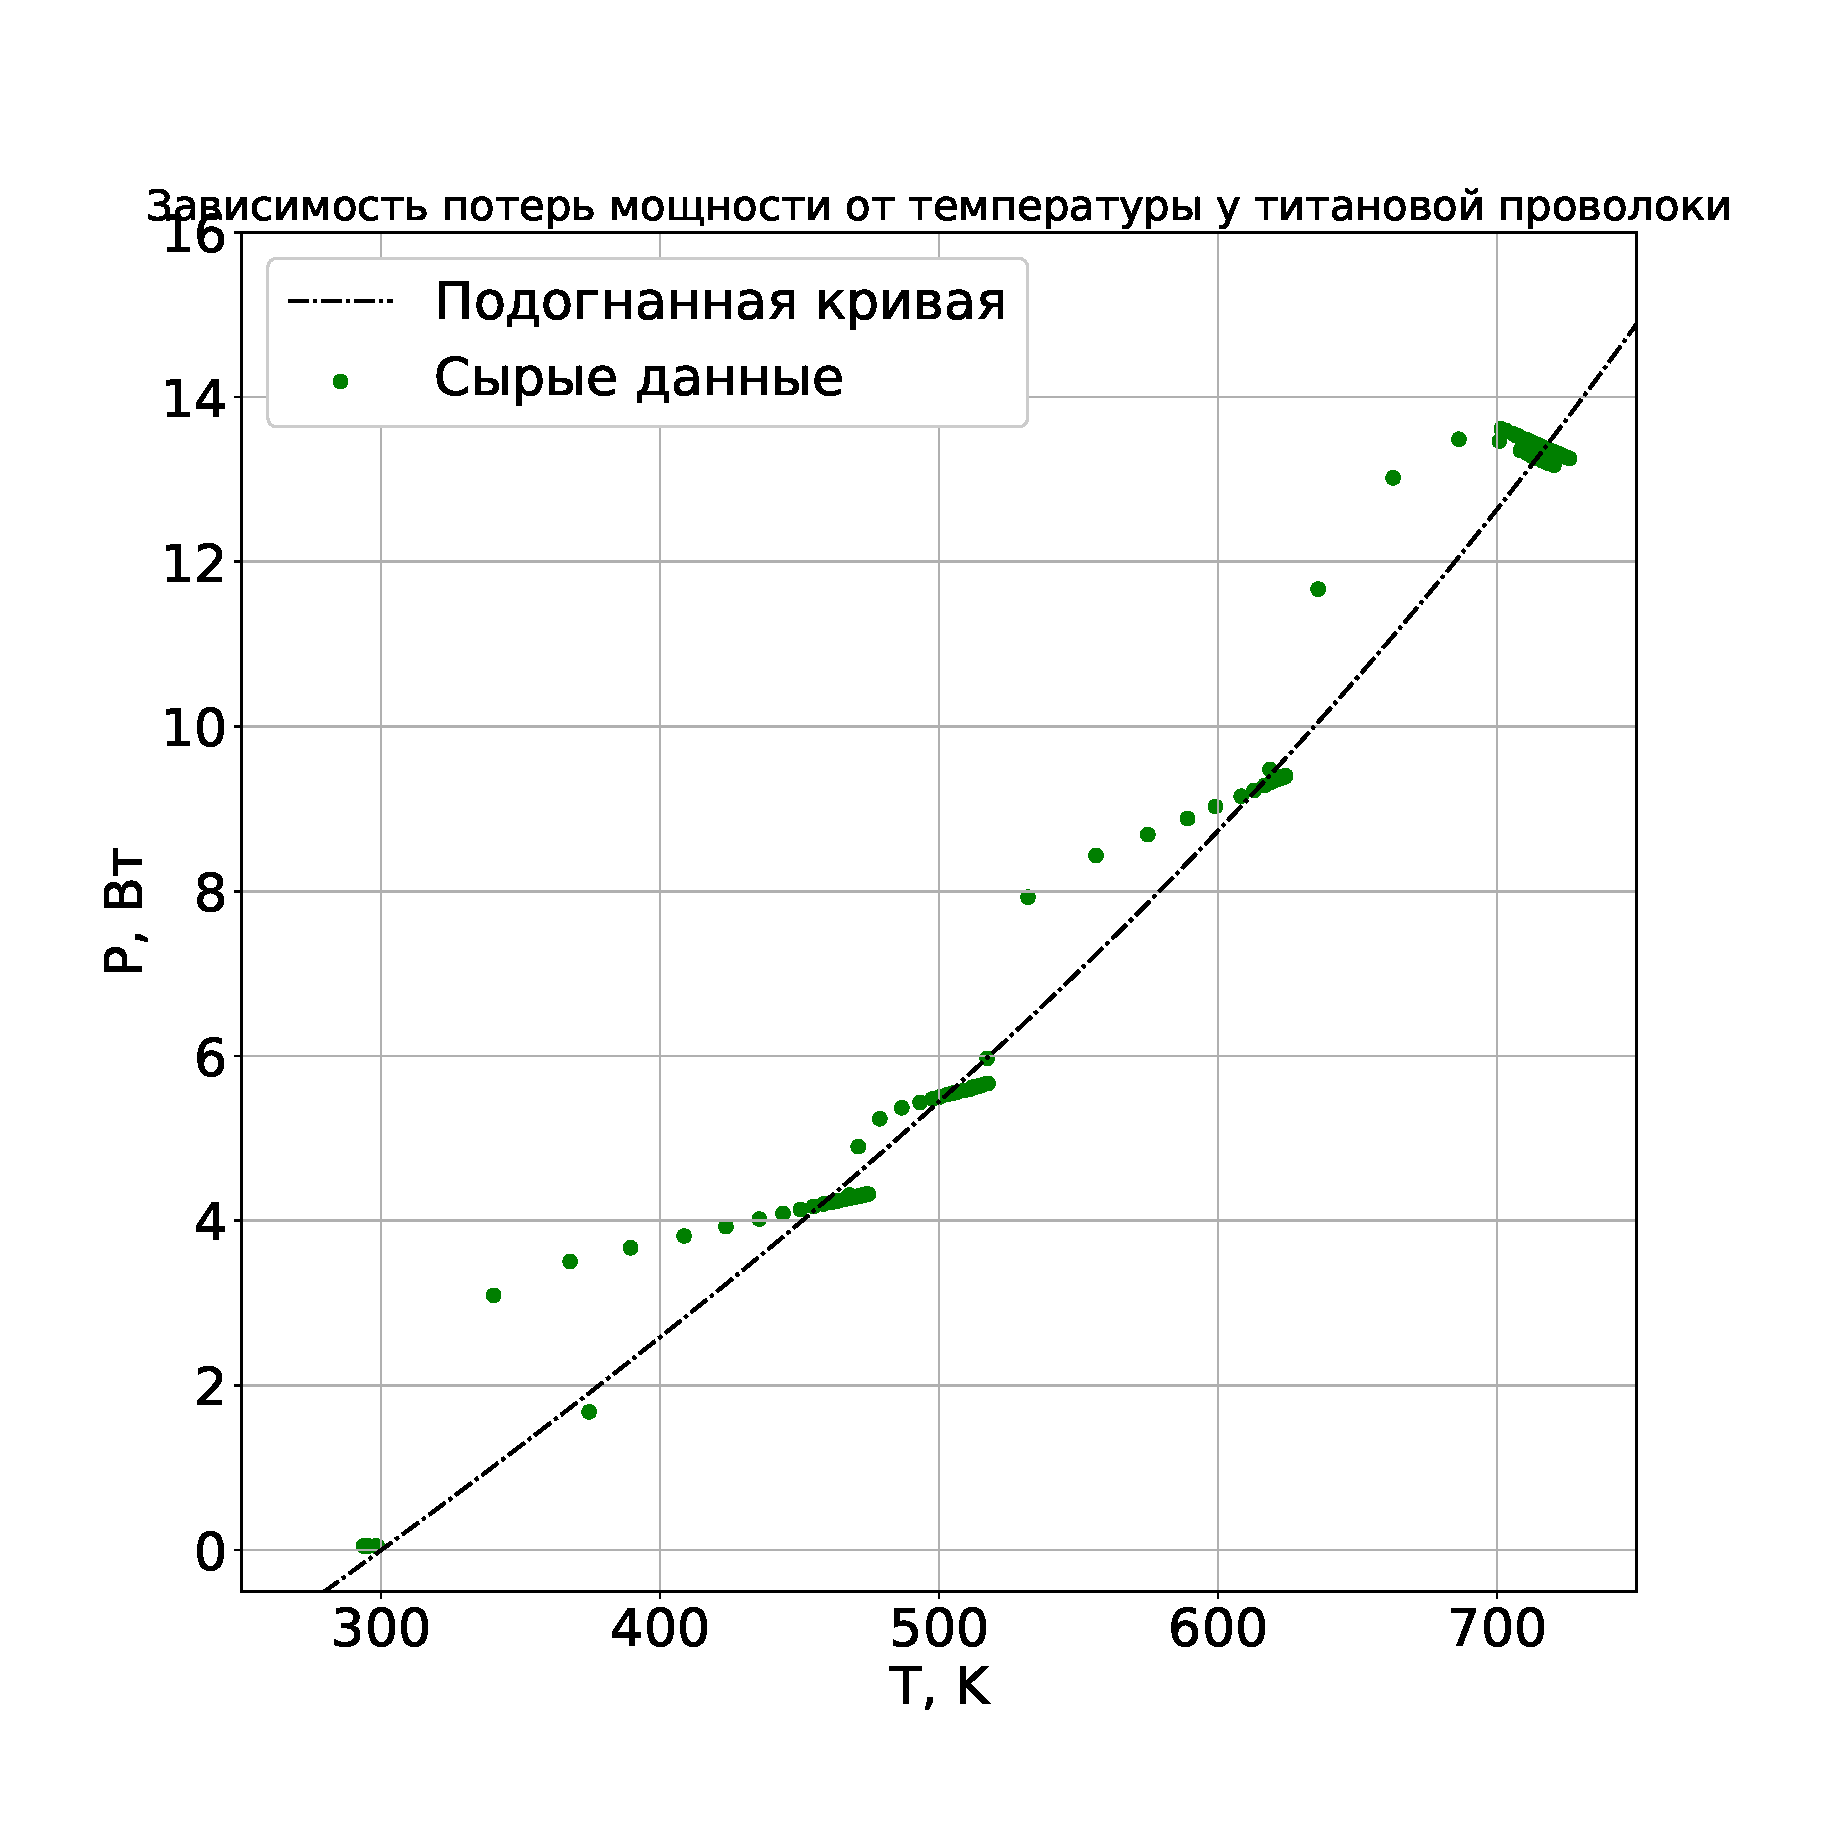
\includegraphics[width=.60\linewidth]{Lab3_7.eps}
				\caption{Коэффициенты $\beta \approx 27$, $\epsilon \approx 0.29$}
				\label{fig}
			\end{figure}
			\begin{figure}[h!]
				\centering
				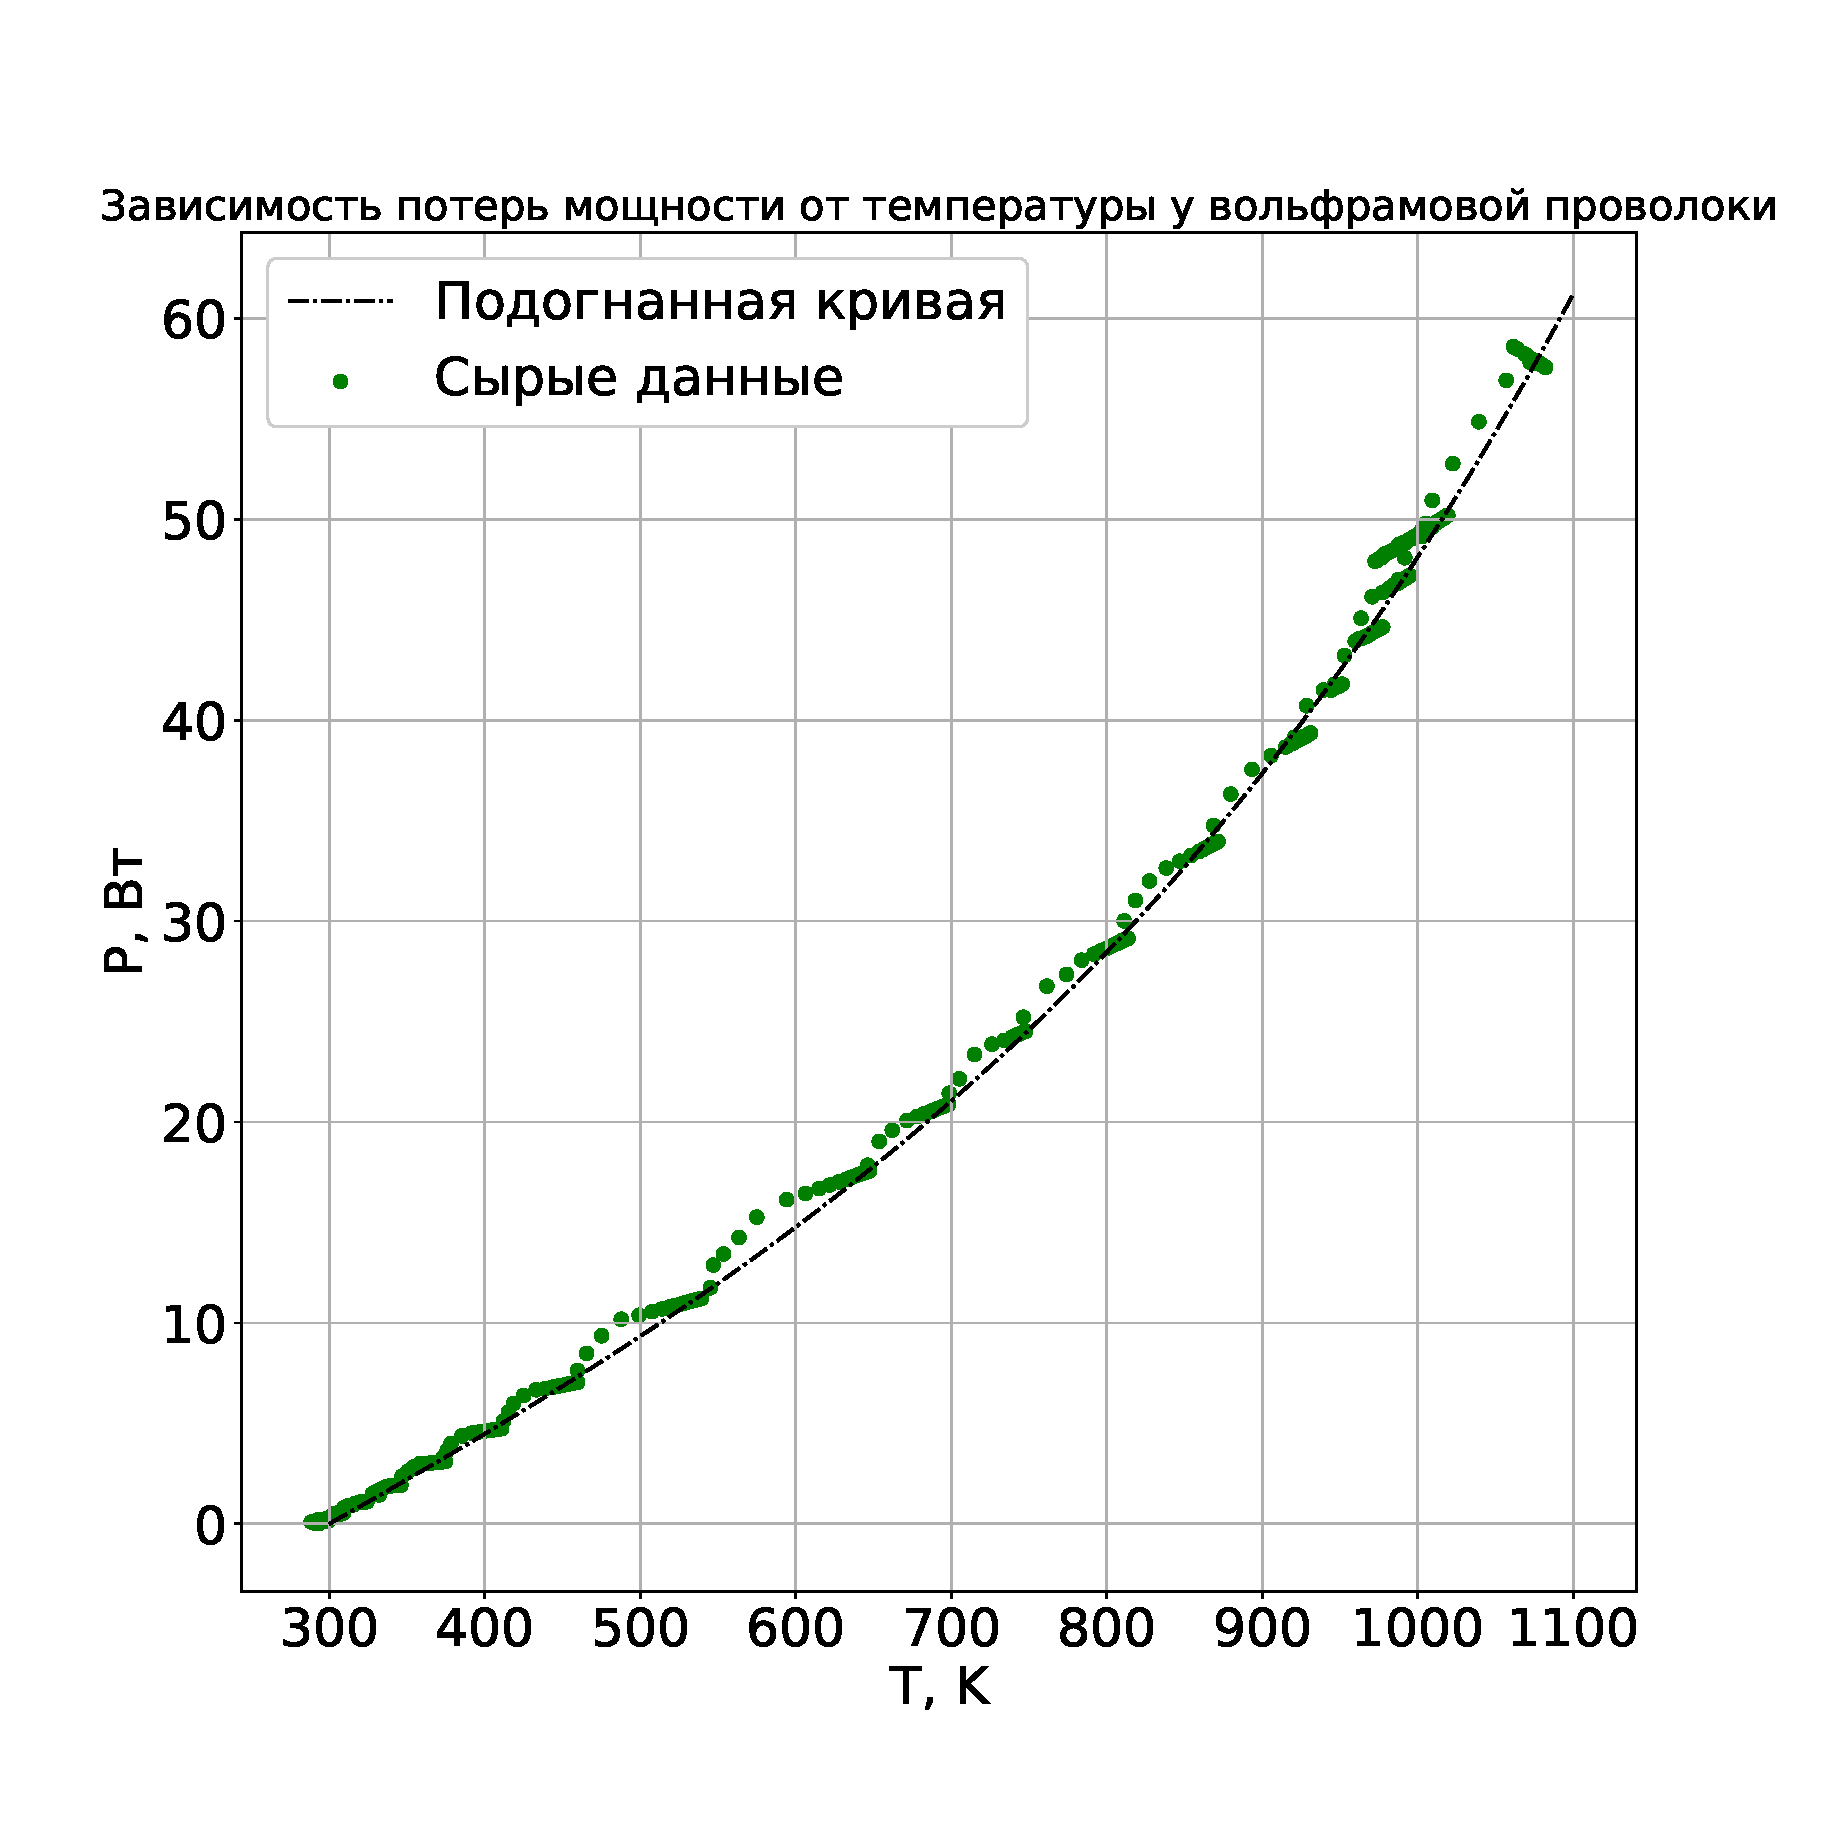
\includegraphics[width=.60\linewidth]{Lab3_8.eps}
				\caption{Коэффициенты $\beta \approx 47.1$, $\epsilon \approx 0.38$}
				\label{fig8}
			\end{figure}
			Теплоемкость была посчитана в предположении, что энергия линейна по температуре и вся мощность уходит на нагрев образца (рассчеты произведены на низких температурах):
				\begin{equation}
				\begin{gathered}
				C_{Cu} = \frac{P \delta t}{m \delta T} \approx 405 \frac{\text{кДж}}{\text{кг} \cdot \text{г}} \\
				C_{Ti} = \frac{P \delta t}{m \delta T} \approx 570 \frac{\text{кДж}}{\text{кг} \cdot \text{г}} \\
				C_{W} = \frac{P \delta t}{m \delta T} \approx 150 \frac{\text{кДж}}{\text{кг} \cdot \text{г}}
				\end{gathered}
				\end{equation}
	\section{Исследование теплоемкости меди}
		\subsection{Ход работы}
			Для того чтобы найти зависимость теплоемкости от температуры воспользуемся другим способом. Известно, что сопротивление при скачке тока меняется по закону $R(t) = R(t_0) + A(1 - \exp(-(t-t_0)/\tau))$. Решая уравнение теплопроводности, выразим коэффициенты через известные нам величины. Таким образом: $R(t) = 1 + \alpha (T_2 - T_1) (1 - \exp(-\frac{(t - t_0)I^2 R(t_0)}{V c (T_2-T_1)})$. Далее будем брать небольшие участки, на которых сопротивление меняется скачком, подгонять для них кривые $R(t)$ и вычислять теплоемкость как подгоночный коэффициент.
		\subsection{Обработка данных}
			Выведем для начала полный график изменения сопротивления со временем
			\begin{figure}[h!]
				\centering
				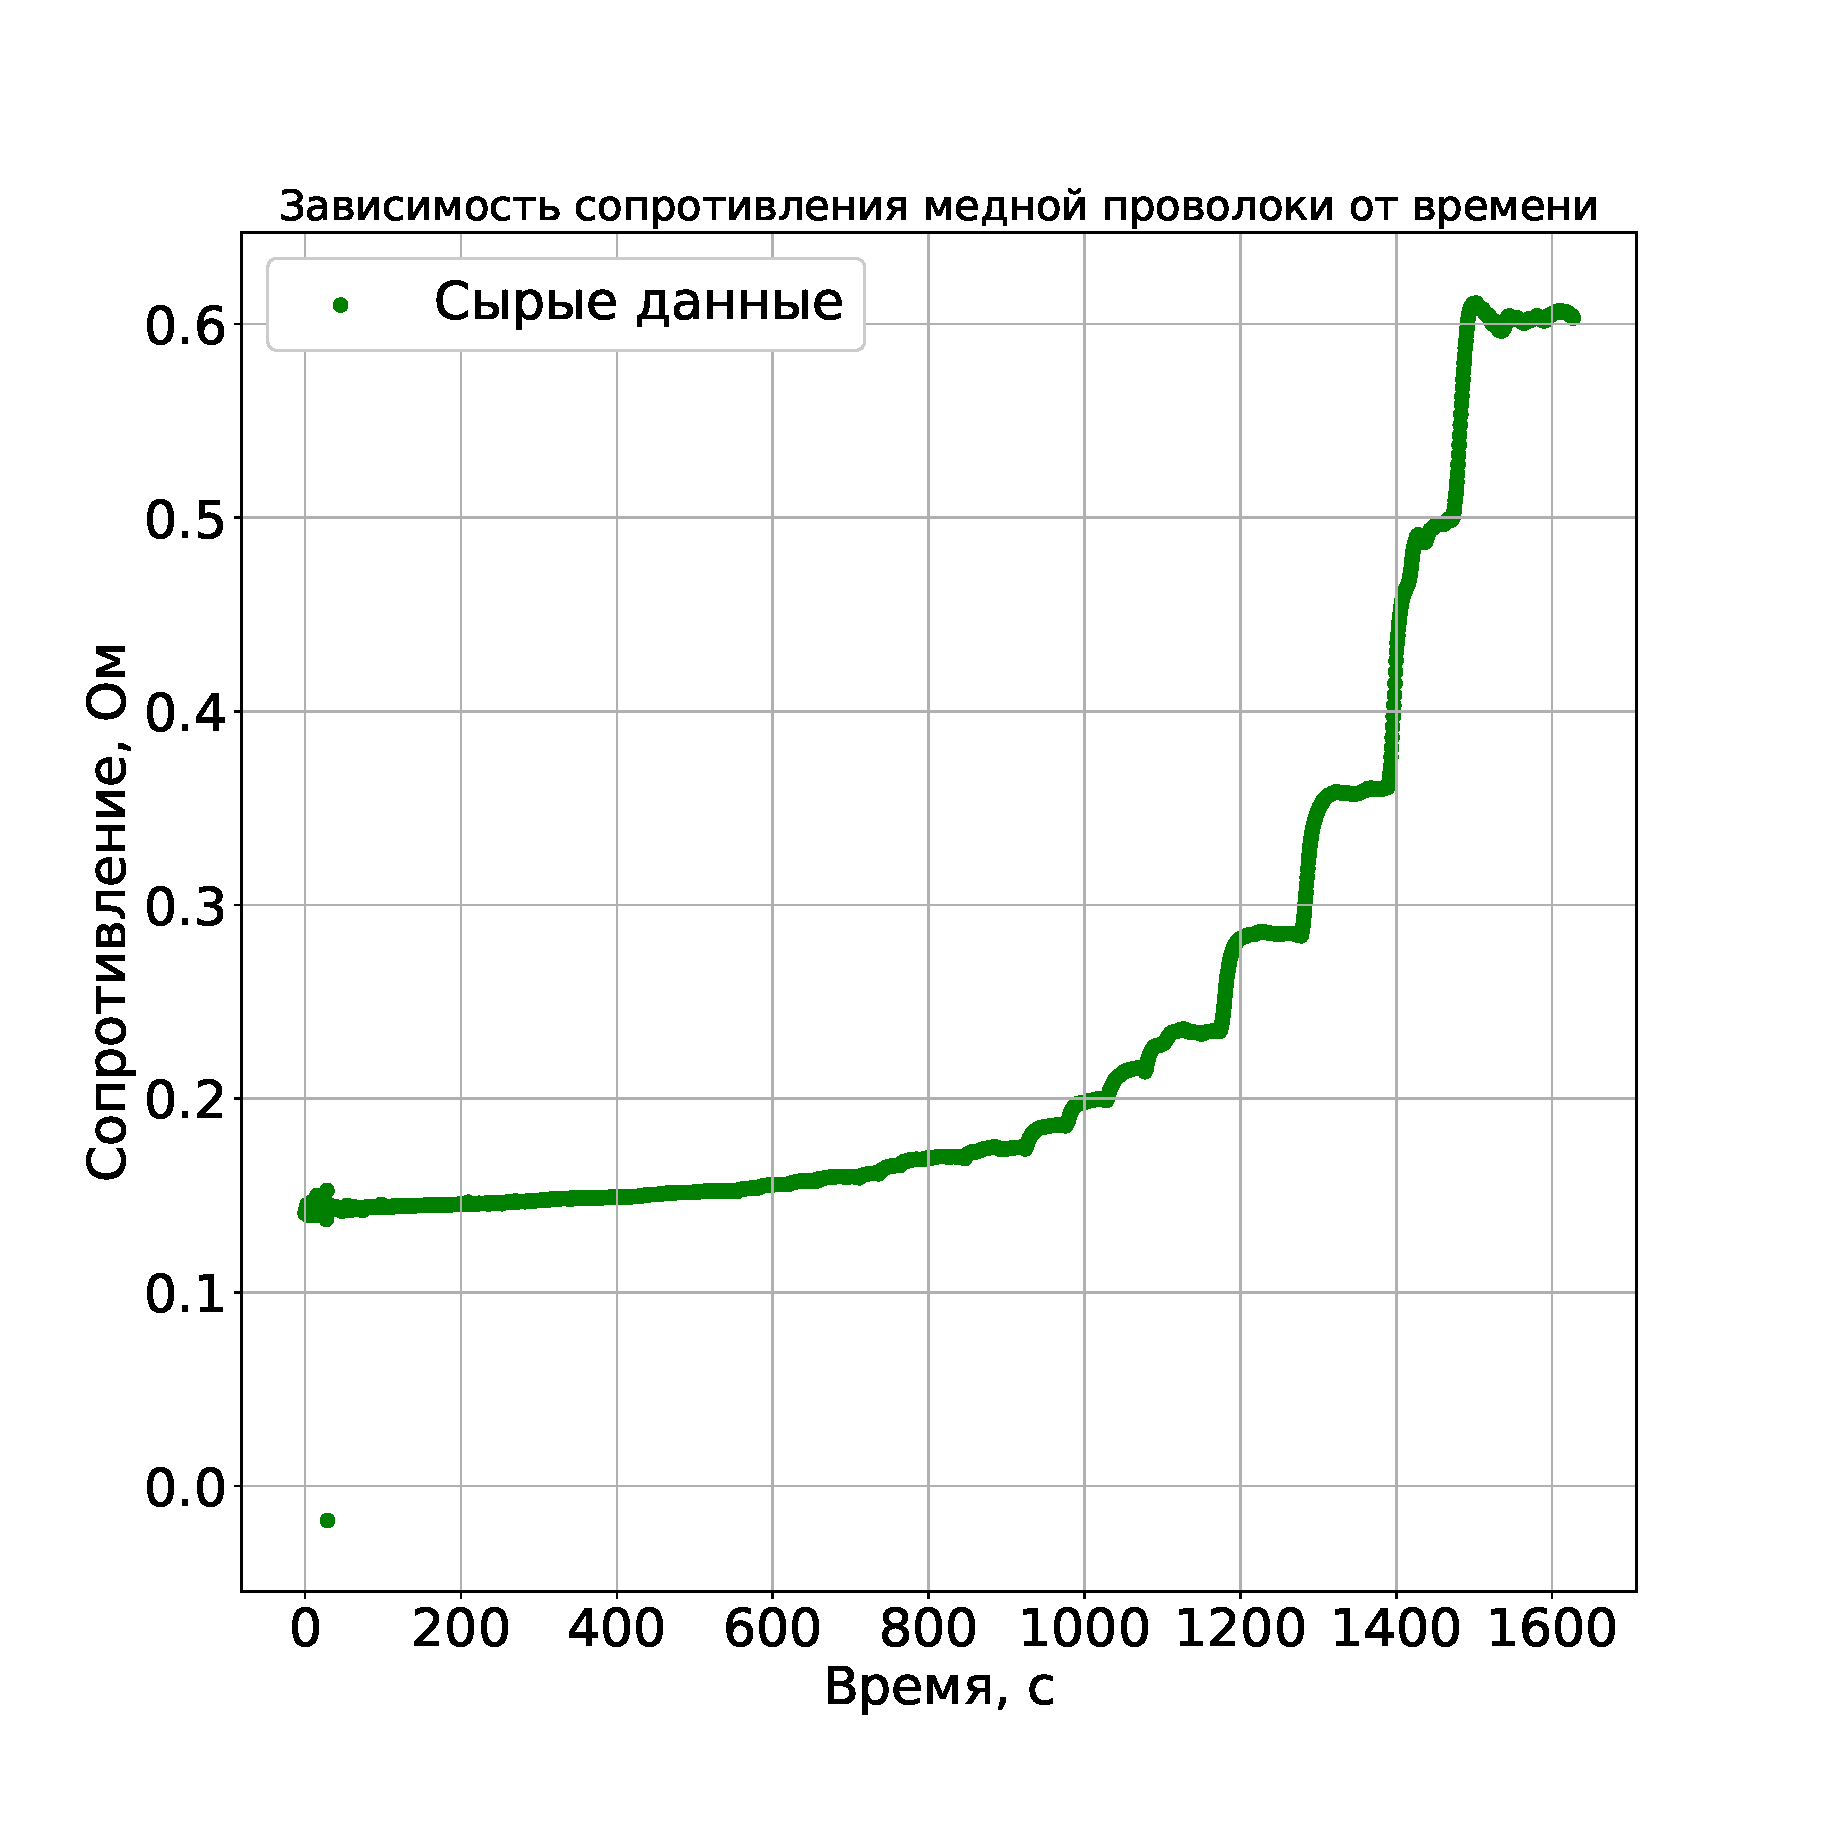
\includegraphics[width=.60\linewidth]{Lab3_14.eps}
				\caption{Изменение сопротивление со временем для медной проволоки}
				\label{fig9}
			\end{figure}
			\newpage
			
			Теперь к каждому отрезку со скачком подгоним кривую для определения теплоемкости.
			\begin{figure}[h!]
				\centering
				\includegraphics[width=.60\linewidth]{Lab3_9.eps}
				\caption{Изменение сопротивление со временем для медной проволоки. Температура $\approx 400K$}
				\label{fig9}
			\end{figure}
			
			\begin{figure}[h!]
				\centering
				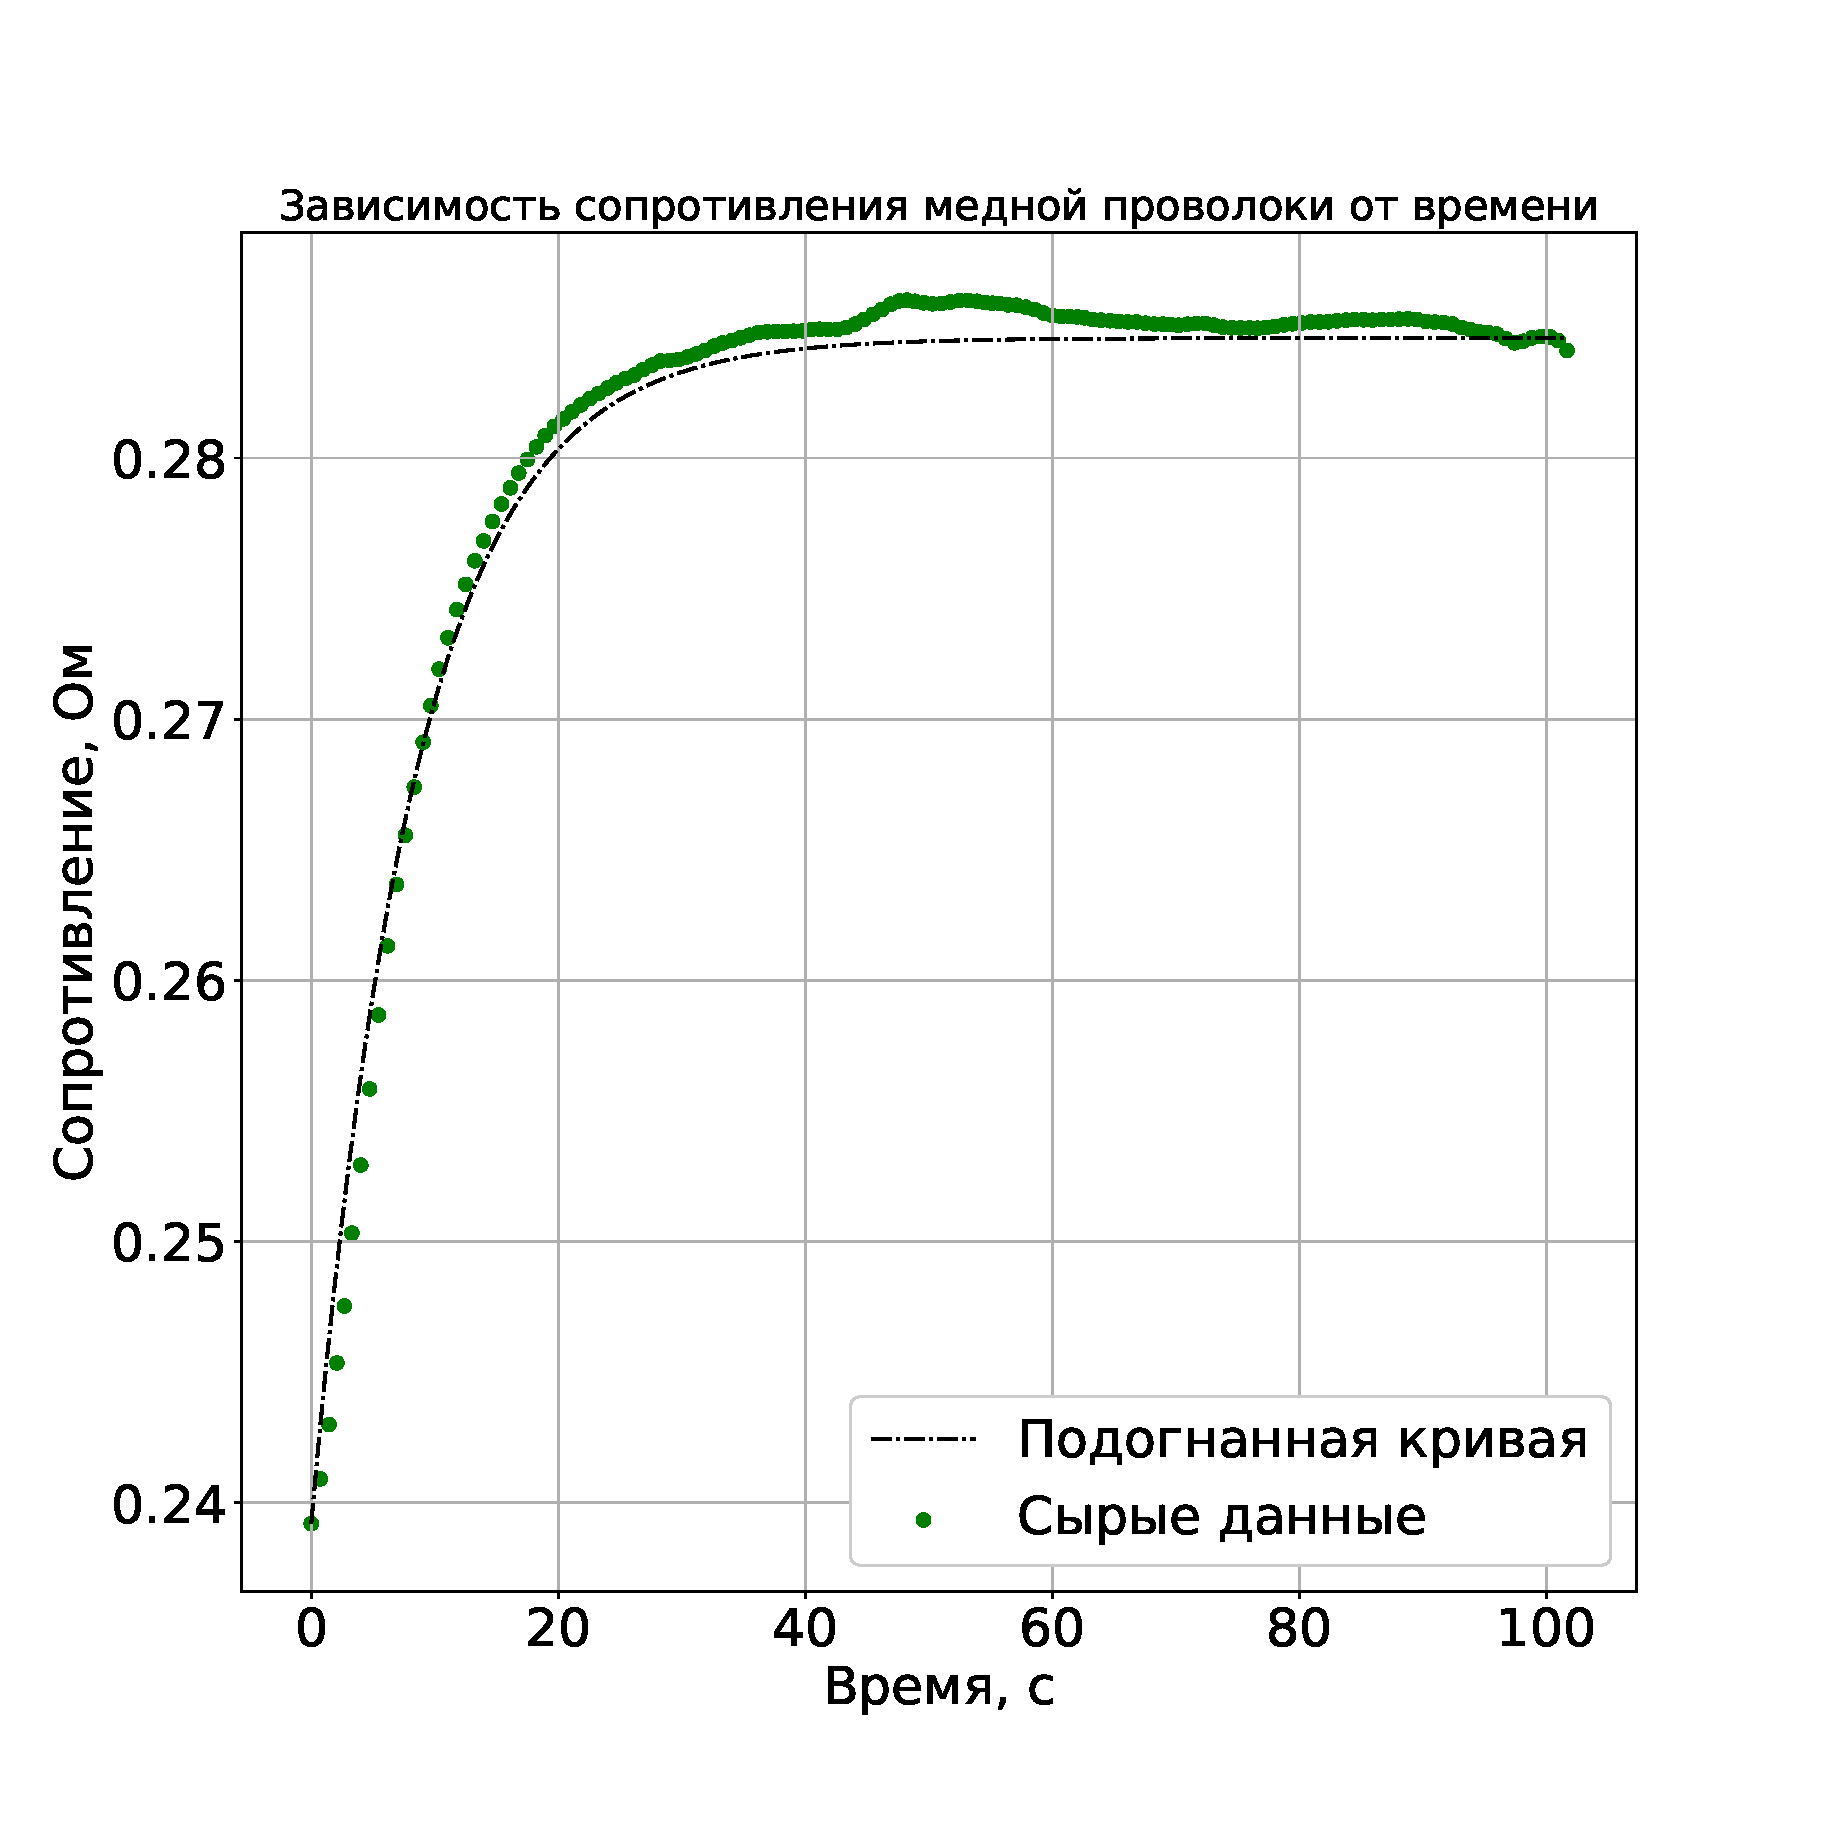
\includegraphics[width=.60\linewidth]{Lab3_10.eps}
				\caption{Изменение сопротивление со временем для медной проволоки. Температура $\approx 480$ К}
				\label{fig9}
			\end{figure}
			
			\begin{figure}[h!]
				\centering
				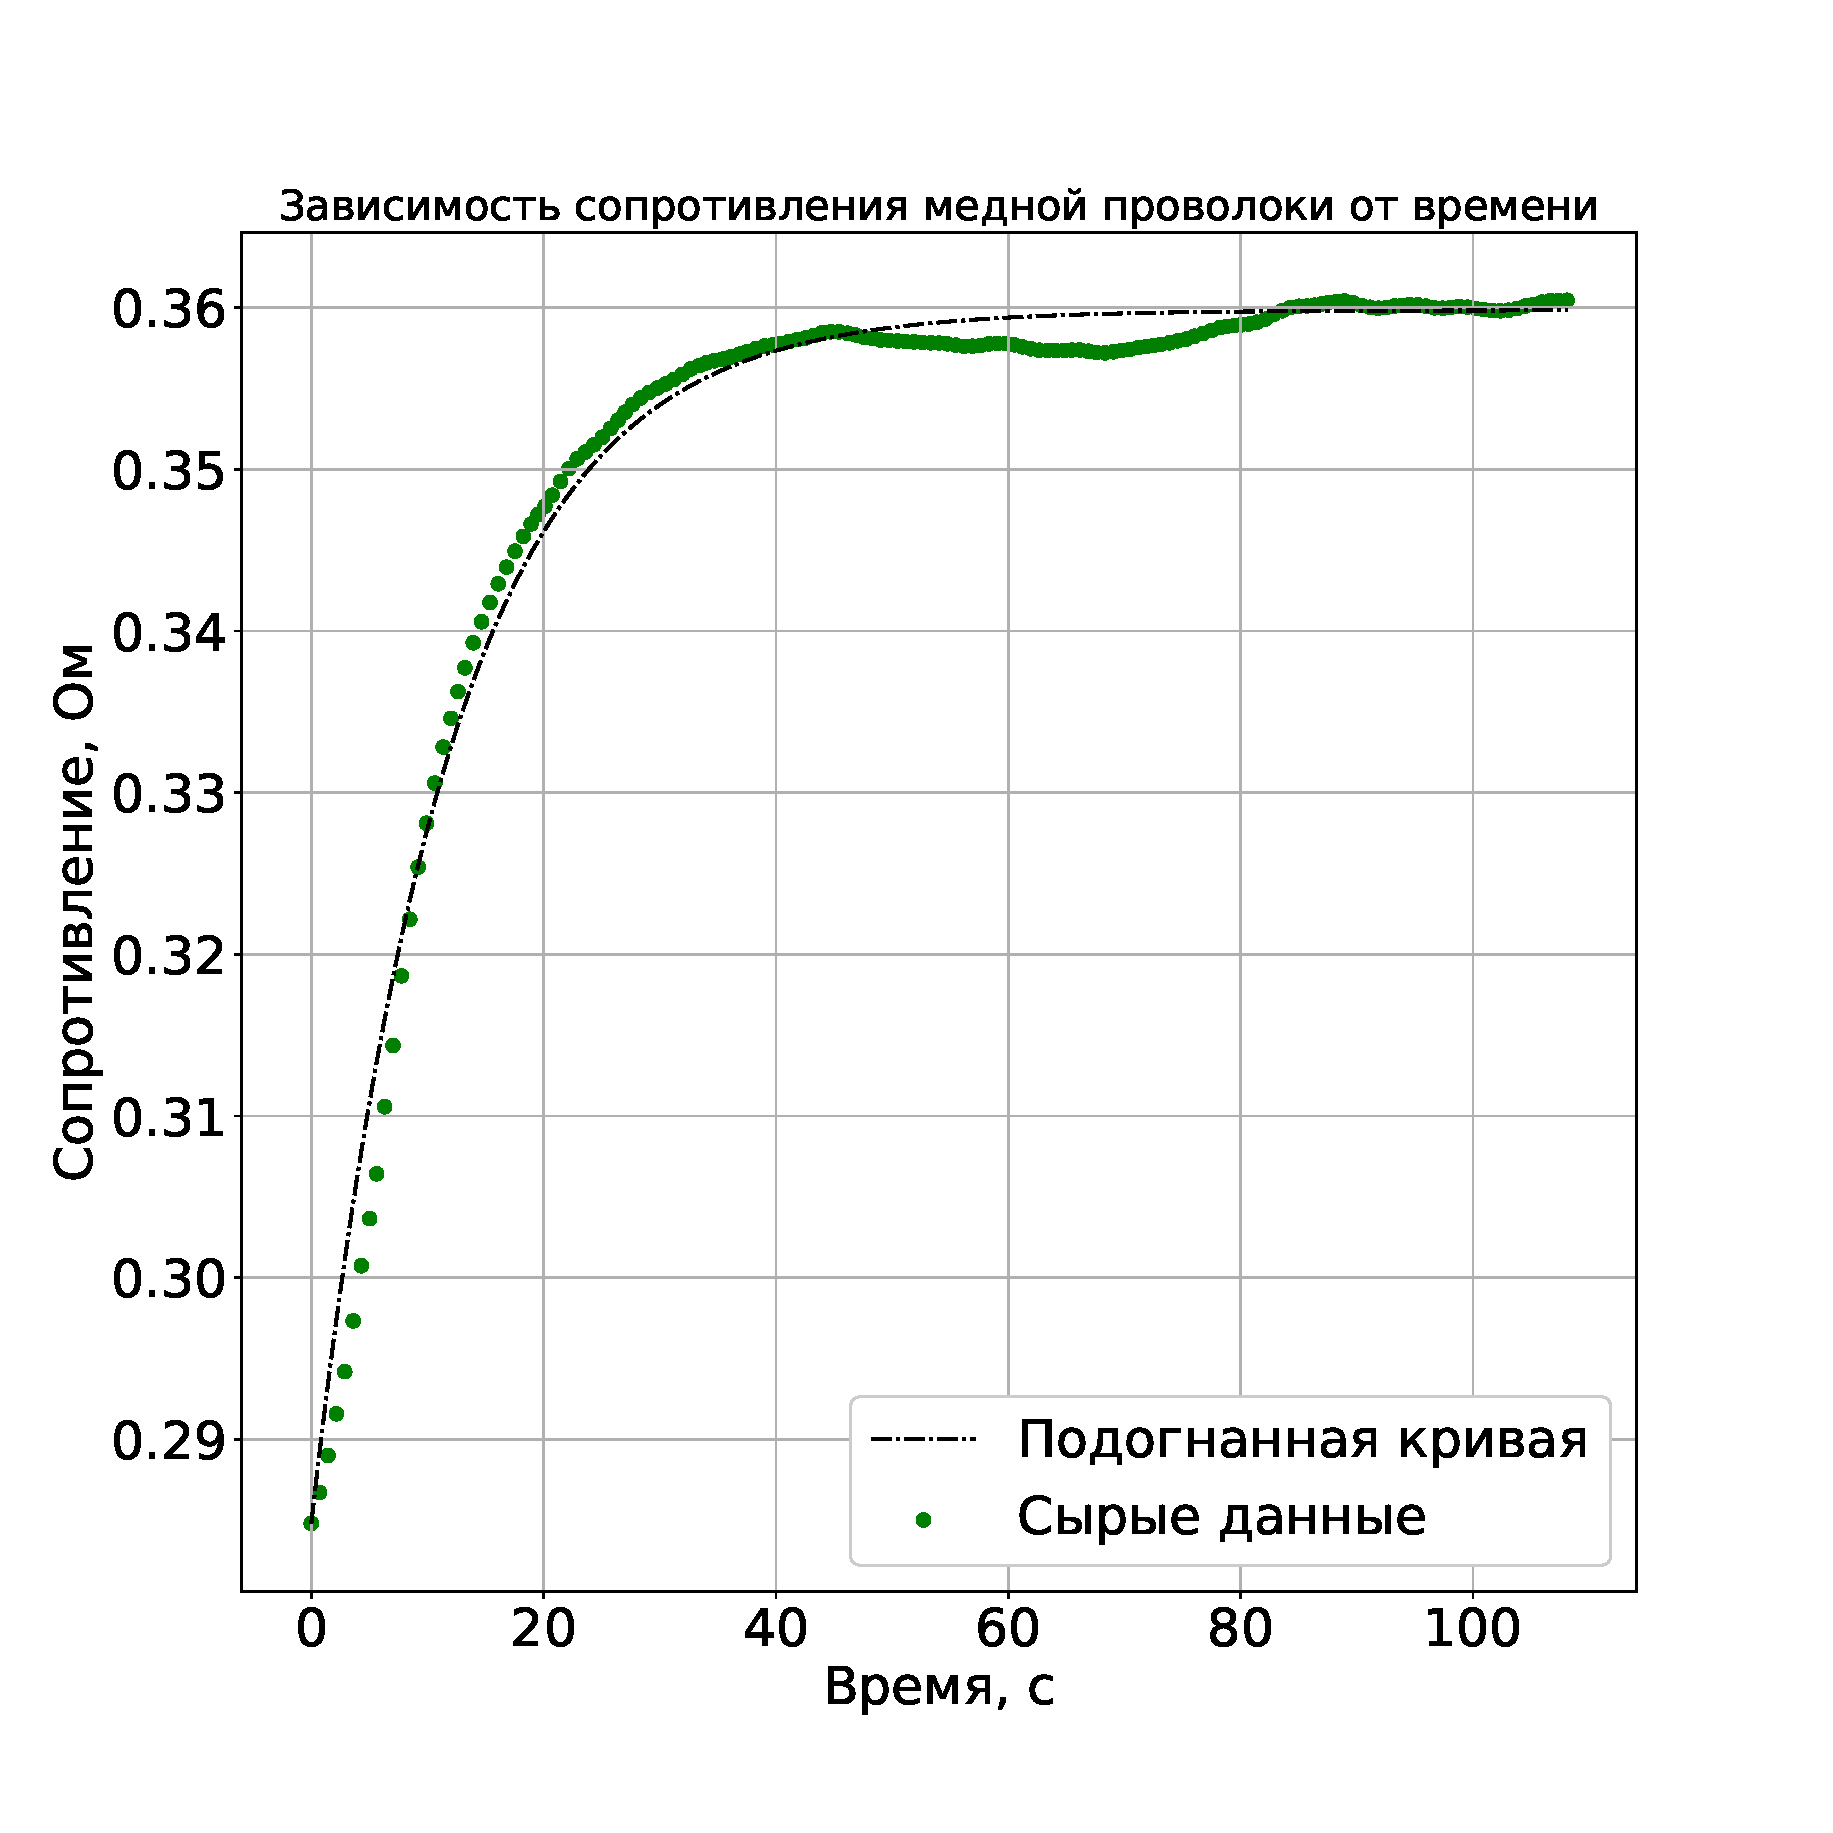
\includegraphics[width=.60\linewidth]{Lab3_11.eps}
				\caption{Изменение сопротивление со временем для медной проволоки. Температура $\approx 570$ К}
				\label{fig9}
			\end{figure}
			
			\begin{figure}[h!]
				\centering
				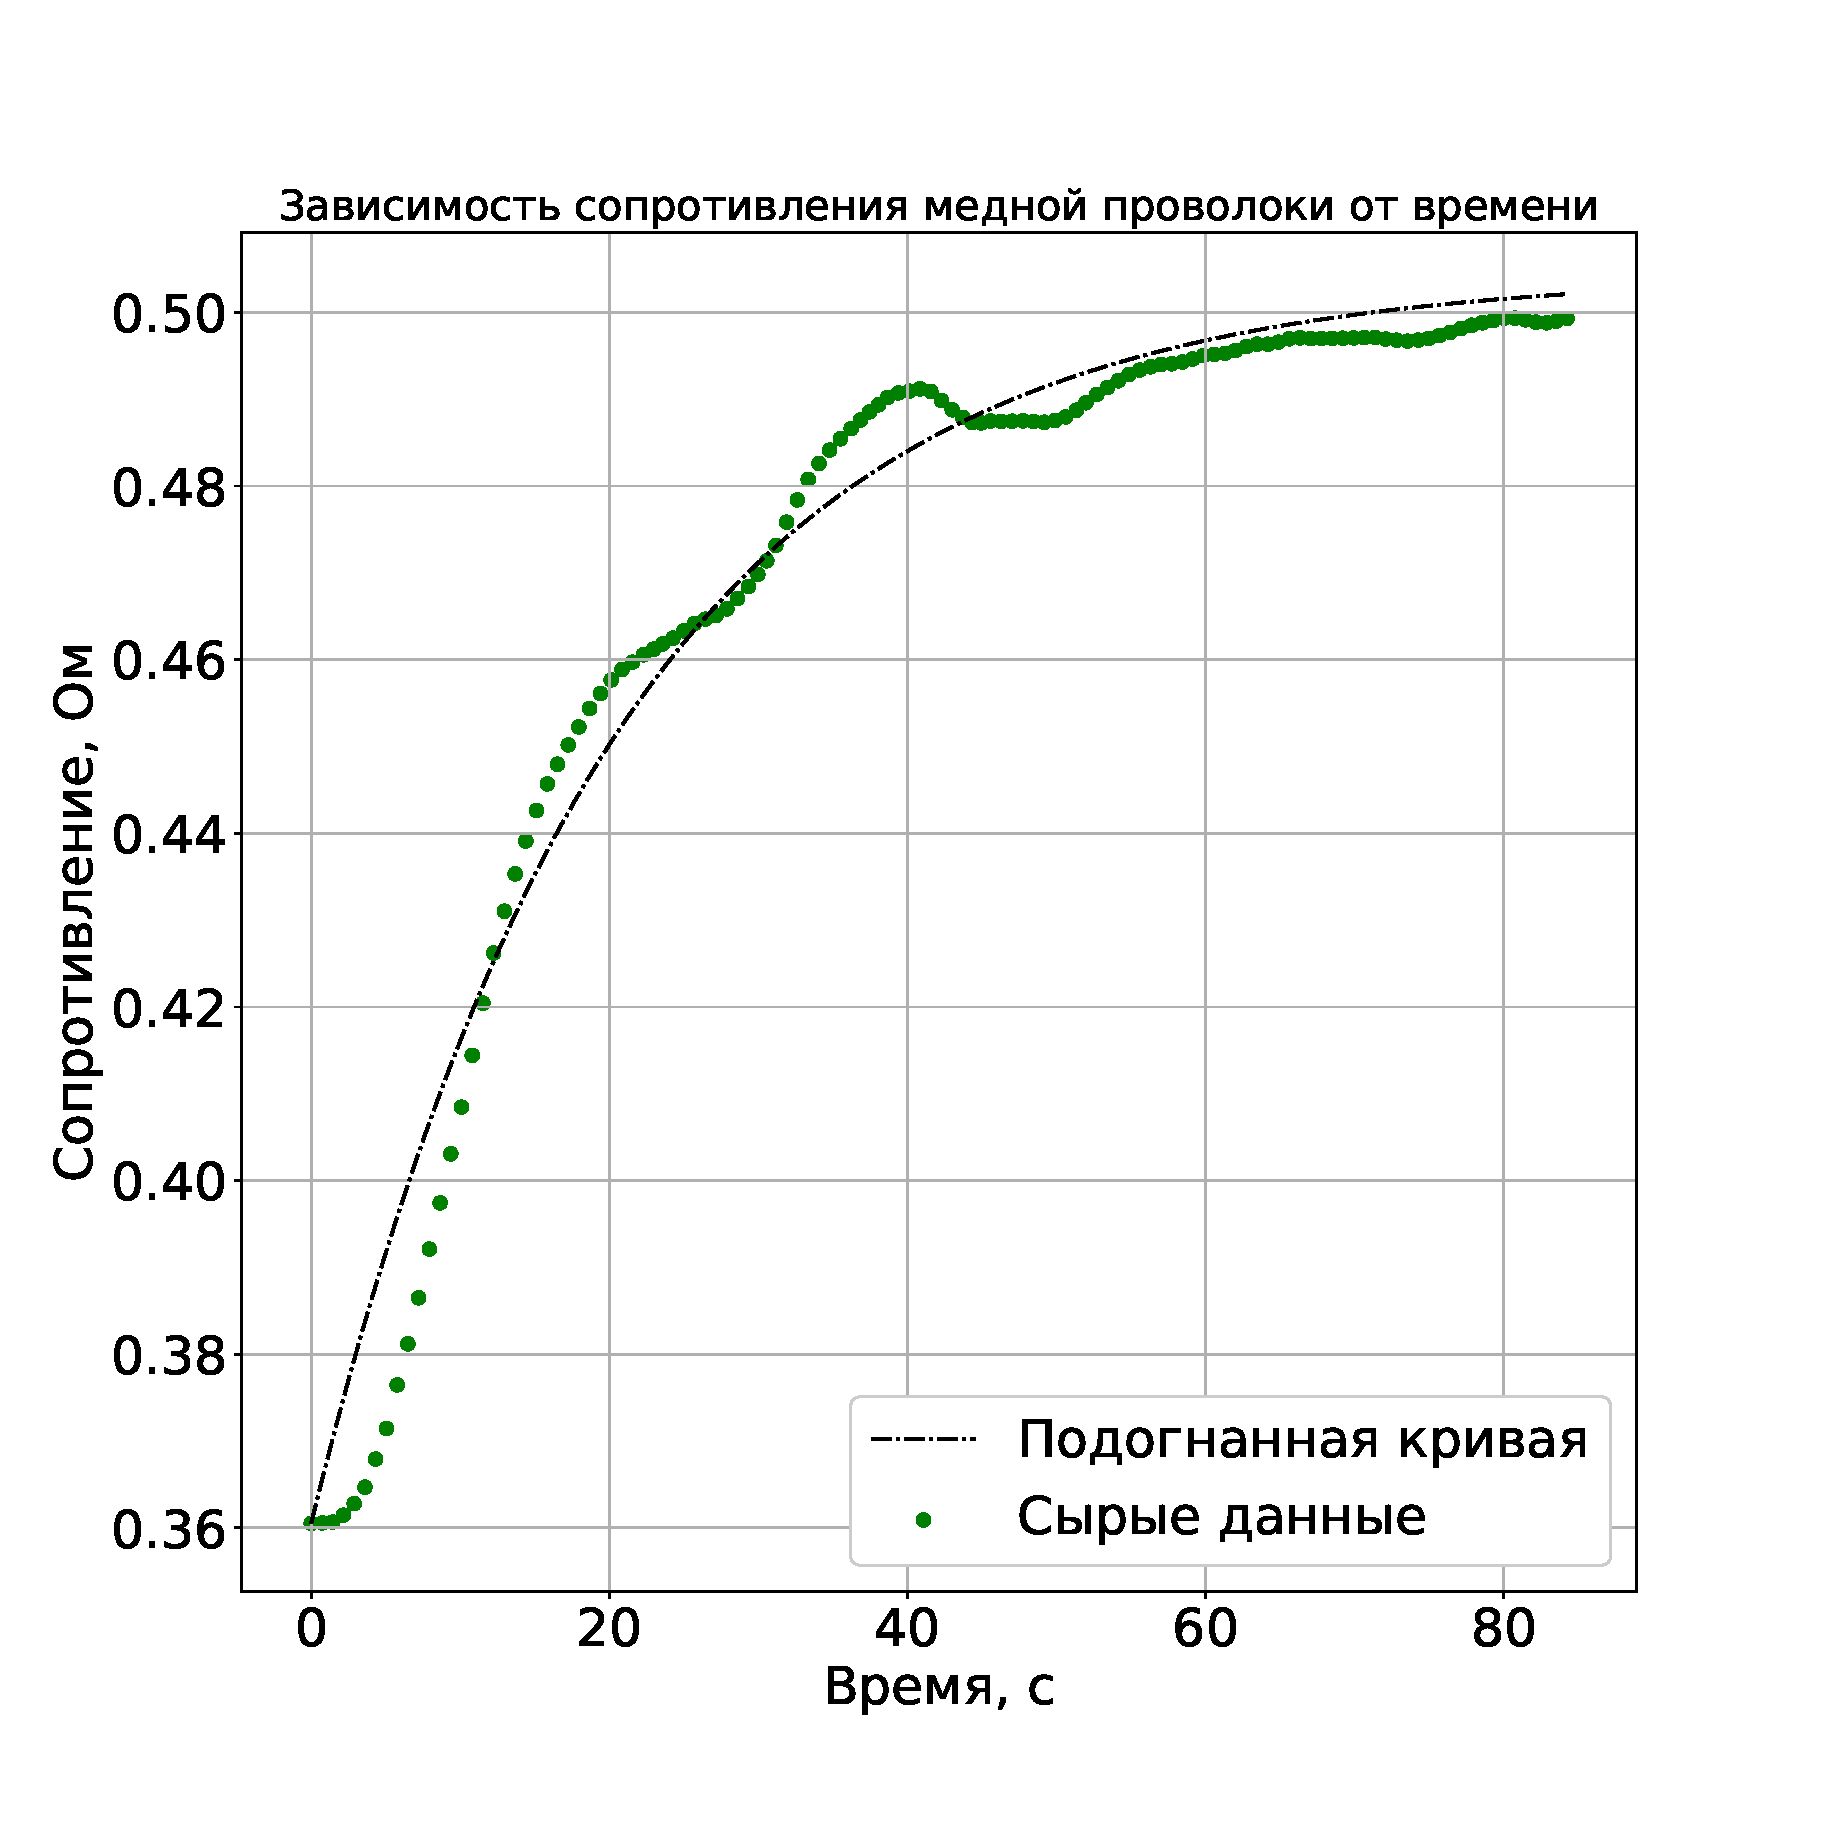
\includegraphics[width=.60\linewidth]{Lab3_12.eps}
				\caption{Изменение сопротивление со временем для медной проволоки. Температура $\approx 650$ К}
				\label{fig9}
			\end{figure}
			\newpage
			
			По полученным данным составим график зависимости удельной теплоемкости меди от температуры
			\begin{figure}[h!]
				\centering
				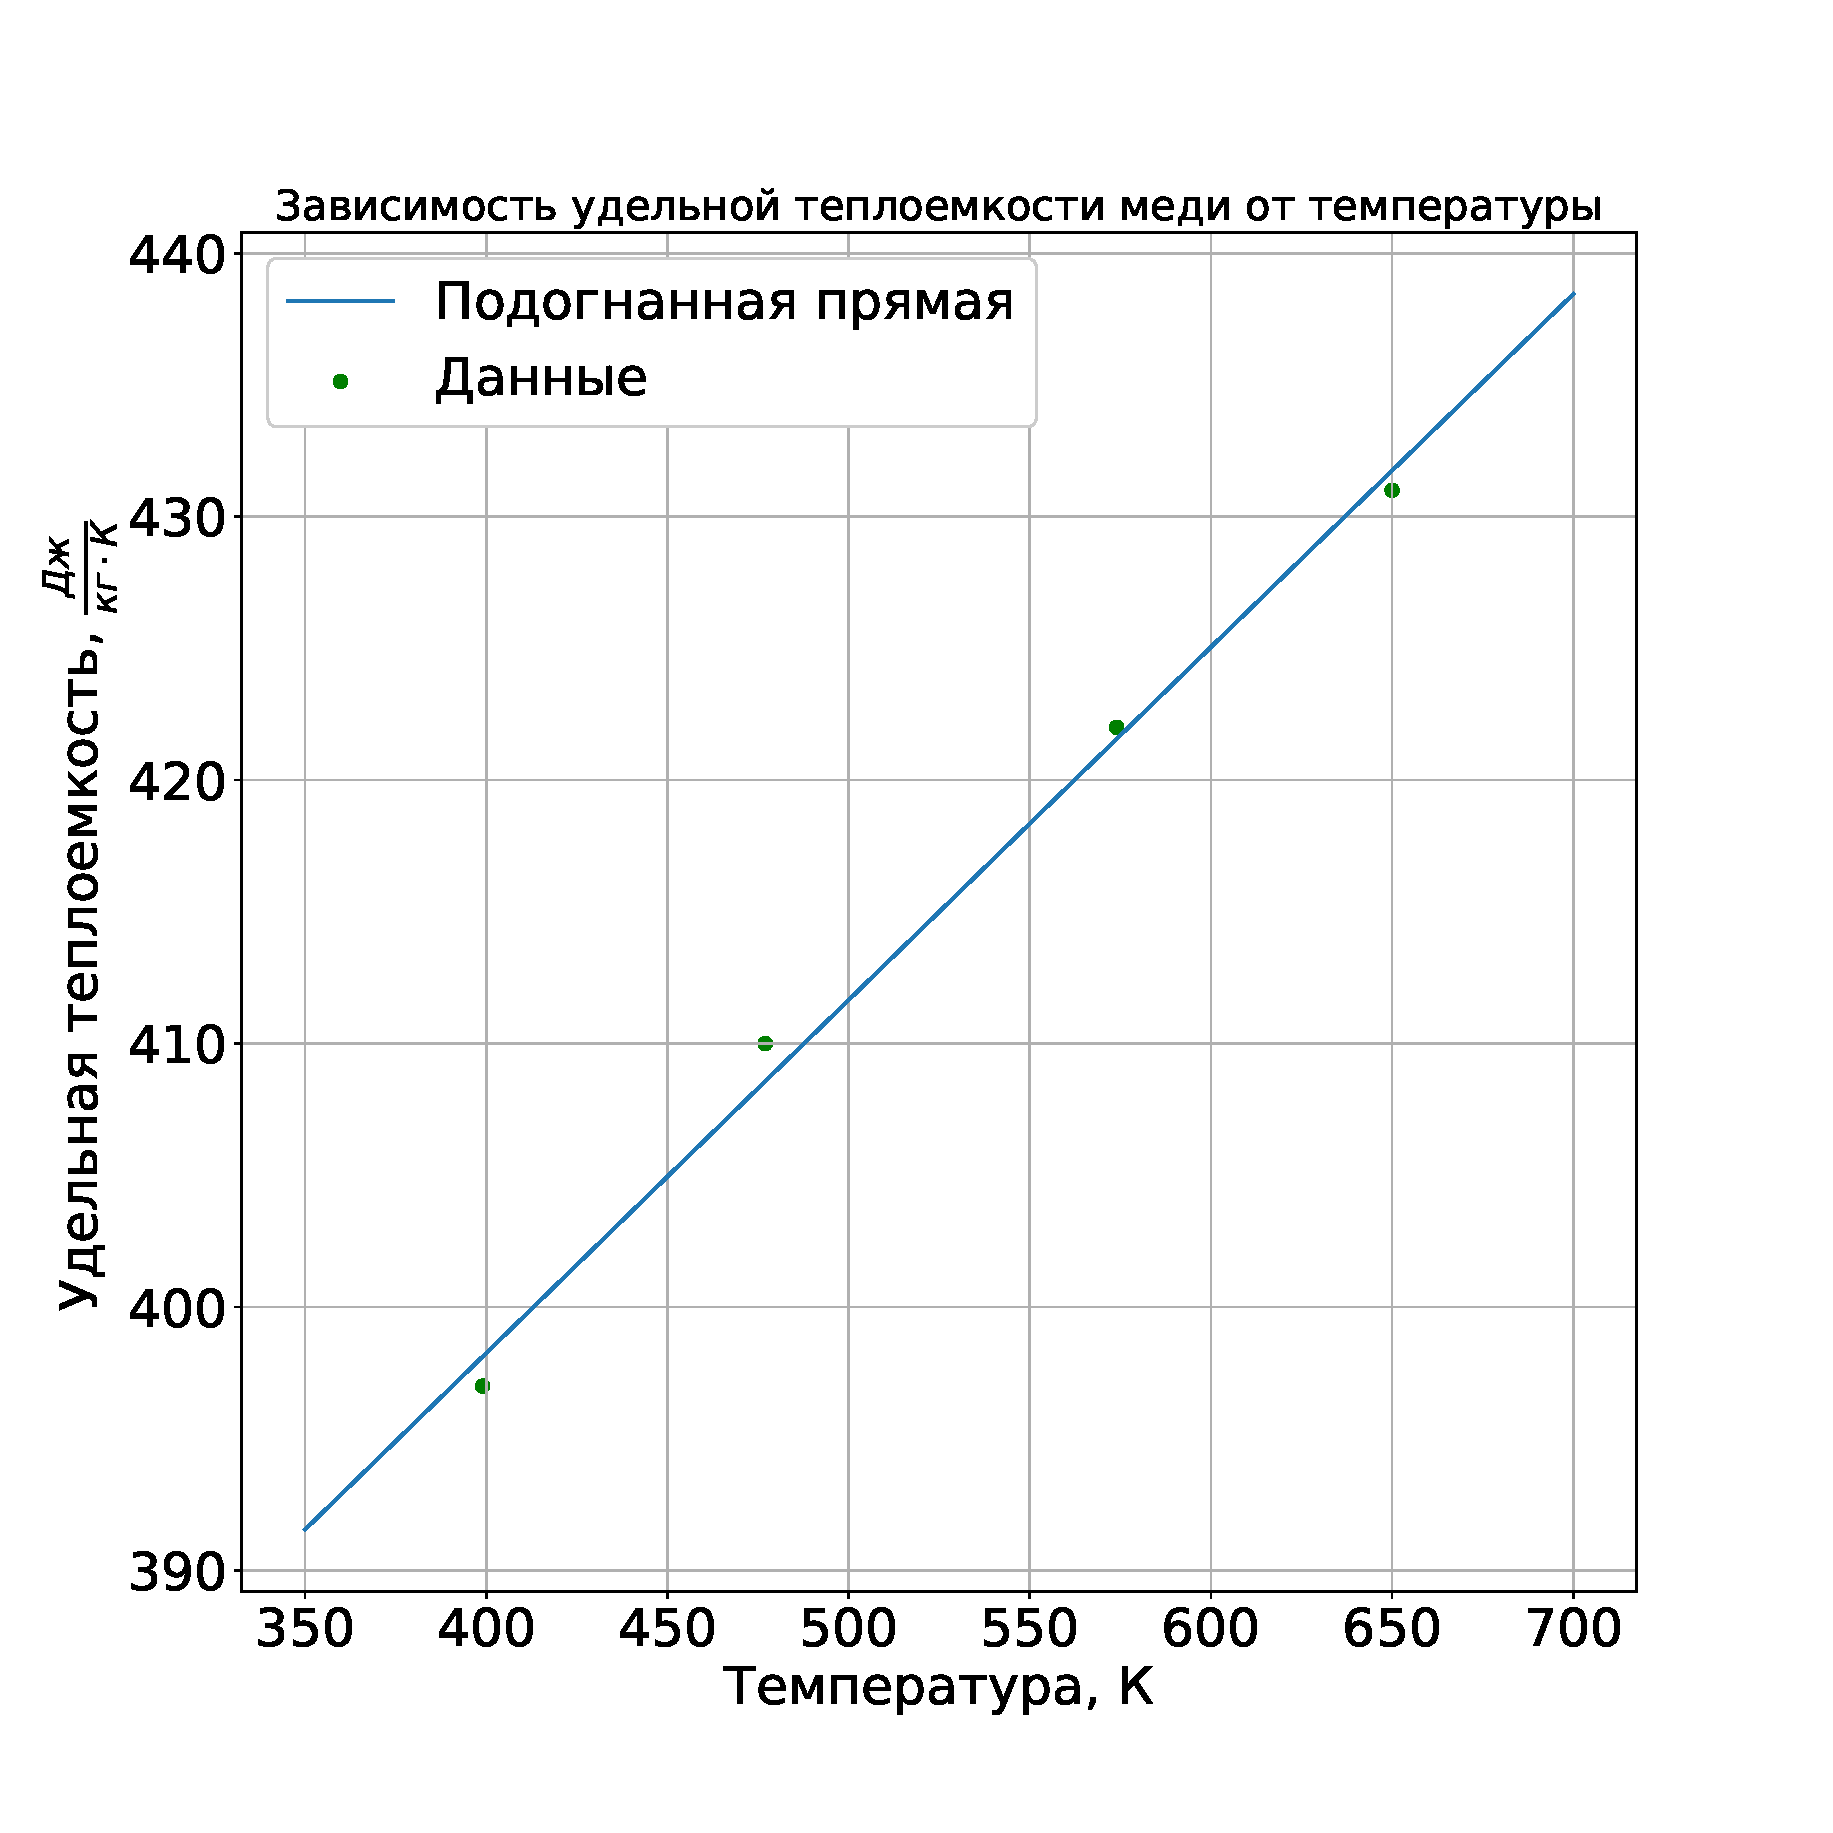
\includegraphics[width=.60\linewidth]{Lab3_13.eps}
				\caption{Изменение теплоемкости с температурой для меди}
				\label{fig9}
			\end{figure}
			
			Как можно видеть, теплоемкость действительно зависит линейно от температуры в таком диапазоне. Коэффициент наклона прямой $\alpha \approx 0.13 \frac{\text{Дж}}{\text{кг} \text{К}^2}$.
\end{document}